\documentclass[twoside]{book}

% Packages required by doxygen
\usepackage{fixltx2e}
\usepackage{calc}
\usepackage{doxygen}
\usepackage[export]{adjustbox} % also loads graphicx
\usepackage{graphicx}
\usepackage[utf8]{inputenc}
\usepackage{makeidx}
\usepackage{multicol}
\usepackage{multirow}
\PassOptionsToPackage{warn}{textcomp}
\usepackage{textcomp}
\usepackage[nointegrals]{wasysym}
\usepackage[table]{xcolor}

% Font selection
\usepackage[T1]{fontenc}
\usepackage[scaled=.90]{helvet}
\usepackage{courier}
\usepackage{amssymb}
\usepackage{sectsty}
\renewcommand{\familydefault}{\sfdefault}
\allsectionsfont{%
  \fontseries{bc}\selectfont%
  \color{darkgray}%
}
\renewcommand{\DoxyLabelFont}{%
  \fontseries{bc}\selectfont%
  \color{darkgray}%
}
\newcommand{\+}{\discretionary{\mbox{\scriptsize$\hookleftarrow$}}{}{}}

% Page & text layout
\usepackage{geometry}
\geometry{%
  a4paper,%
  top=2.5cm,%
  bottom=2.5cm,%
  left=2.5cm,%
  right=2.5cm%
}
\tolerance=750
\hfuzz=15pt
\hbadness=750
\setlength{\emergencystretch}{15pt}
\setlength{\parindent}{0cm}
\setlength{\parskip}{3ex plus 2ex minus 2ex}
\makeatletter
\renewcommand{\paragraph}{%
  \@startsection{paragraph}{4}{0ex}{-1.0ex}{1.0ex}{%
    \normalfont\normalsize\bfseries\SS@parafont%
  }%
}
\renewcommand{\subparagraph}{%
  \@startsection{subparagraph}{5}{0ex}{-1.0ex}{1.0ex}{%
    \normalfont\normalsize\bfseries\SS@subparafont%
  }%
}
\makeatother

% Headers & footers
\usepackage{fancyhdr}
\pagestyle{fancyplain}
\fancyhead[LE]{\fancyplain{}{\bfseries\thepage}}
\fancyhead[CE]{\fancyplain{}{}}
\fancyhead[RE]{\fancyplain{}{\bfseries\leftmark}}
\fancyhead[LO]{\fancyplain{}{\bfseries\rightmark}}
\fancyhead[CO]{\fancyplain{}{}}
\fancyhead[RO]{\fancyplain{}{\bfseries\thepage}}
\fancyfoot[LE]{\fancyplain{}{}}
\fancyfoot[CE]{\fancyplain{}{}}
\fancyfoot[RE]{\fancyplain{}{\bfseries\scriptsize Generated by Doxygen }}
\fancyfoot[LO]{\fancyplain{}{\bfseries\scriptsize Generated by Doxygen }}
\fancyfoot[CO]{\fancyplain{}{}}
\fancyfoot[RO]{\fancyplain{}{}}
\renewcommand{\footrulewidth}{0.4pt}
\renewcommand{\chaptermark}[1]{%
  \markboth{#1}{}%
}
\renewcommand{\sectionmark}[1]{%
  \markright{\thesection\ #1}%
}

% Indices & bibliography
\usepackage{natbib}
\usepackage[titles]{tocloft}
\setcounter{tocdepth}{3}
\setcounter{secnumdepth}{5}
\makeindex

% Hyperlinks (required, but should be loaded last)
\usepackage{ifpdf}
\ifpdf
  \usepackage[pdftex,pagebackref=true]{hyperref}
\else
  \usepackage[ps2pdf,pagebackref=true]{hyperref}
\fi
\hypersetup{%
  colorlinks=true,%
  linkcolor=blue,%
  citecolor=blue,%
  unicode%
}

% Custom commands
\newcommand{\clearemptydoublepage}{%
  \newpage{\pagestyle{empty}\cleardoublepage}%
}

\usepackage{caption}
\captionsetup{labelsep=space,justification=centering,font={bf},singlelinecheck=off,skip=4pt,position=top}

%===== C O N T E N T S =====

\begin{document}

% Titlepage & ToC
\hypersetup{pageanchor=false,
             bookmarksnumbered=true,
             pdfencoding=unicode
            }
\pagenumbering{roman}
\begin{titlepage}
\vspace*{7cm}
\begin{center}%
{\Large My Project }\\
\vspace*{1cm}
{\large Generated by Doxygen 1.8.11}\\
\end{center}
\end{titlepage}
\clearemptydoublepage
\tableofcontents
\clearemptydoublepage
\pagenumbering{arabic}
\hypersetup{pageanchor=true}

%--- Begin generated contents ---
\chapter{Class Index}
\section{Class List}
Here are the classes, structs, unions and interfaces with brief descriptions\+:\begin{DoxyCompactList}
\item\contentsline{section}{\hyperlink{structnode}{node} }{\pageref{structnode}}{}
\item\contentsline{section}{\hyperlink{structnode1}{node1} }{\pageref{structnode1}}{}
\item\contentsline{section}{\hyperlink{structnode__info}{node\+\_\+info} }{\pageref{structnode__info}}{}
\end{DoxyCompactList}

\chapter{File Index}
\section{File List}
Here is a list of all files with brief descriptions\+:\begin{DoxyCompactList}
\item\contentsline{section}{\hyperlink{Lab1_8c}{Lab1.\+c} }{\pageref{Lab1_8c}}{}
\end{DoxyCompactList}

\chapter{Class Documentation}
\hypertarget{classLinkedList}{}\section{Linked\+List$<$ T $>$ Class Template Reference}
\label{classLinkedList}\index{Linked\+List$<$ T $>$@{Linked\+List$<$ T $>$}}


{\ttfamily \#include $<$Linked\+List.\+h$>$}



Inheritance diagram for Linked\+List$<$ T $>$\+:
\nopagebreak
\begin{figure}[H]
\begin{center}
\leavevmode
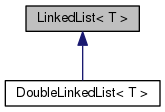
\includegraphics[width=196pt]{classLinkedList__inherit__graph}
\end{center}
\end{figure}
\subsection*{Public Member Functions}
\begin{DoxyCompactItemize}
\item 
\hyperlink{classLinkedList_a3c20fcfec867e867f541061a09fc640c}{Linked\+List} ()
\item 
\hyperlink{classLinkedList_a6d0ec2b365564af3f855d245a85bcbef}{Linked\+List} (const \hyperlink{classLinkedList}{Linked\+List}$<$ T $>$ \&l, bool sort=false)
\item 
\hyperlink{classLinkedList_a7c37609df3b83bc4eb0281b852f93fd7}{$\sim$\+Linked\+List} ()
\item 
int \hyperlink{classLinkedList_ae04dbbcae32f8fb03dce3e174854981f}{get\+Num\+Node} () const 
\item 
\hyperlink{classNode}{Node}$<$ T $>$ $\ast$ \hyperlink{classLinkedList_af59e26b062e8e9549974adfa5bb51eb2}{get\+Head} () const 
\item 
virtual void \hyperlink{classLinkedList_ac2f92598858e9ba02af8722fba803c53}{append} (\hyperlink{classNode}{Node}$<$ T $>$ $\ast$n)
\item 
virtual void \hyperlink{classLinkedList_a62a89a30509d38b88c75177b8efa9a98}{delete\+At\+Pos} (int pos)
\item 
void \hyperlink{classLinkedList_afddb5dbcc39e687add40de41b975cd8d}{display} () const 
\item 
void \hyperlink{classLinkedList_a7ed3bb4986b76cbfd3547d0b262ffff3}{display\+Node} (\hyperlink{classNode}{Node}$<$ T $>$ $\ast$curr) const 
\item 
bool \hyperlink{classLinkedList_a1b28b1e19e5aa68f3d89352e307928f6}{is\+Empty} () const 
\item 
void \hyperlink{classLinkedList_a718246359a2199be67212703be951071}{insert} (\hyperlink{classNode}{Node}$<$ T $>$ $\ast$n)
\item 
virtual void \hyperlink{classLinkedList_aa7b12c5f9bb22be91012d68c9da0b431}{insert\+At\+Pos} (\hyperlink{classNode}{Node}$<$ T $>$ $\ast$n, int pos)
\item 
void \hyperlink{classLinkedList_aa644d66bfb879e71d1805a794a78b928}{bubble\+Sort} ()
\item 
void \hyperlink{classLinkedList_abd329a83adcec046dc482f7566cf91f4}{selection\+Sort} ()
\item 
void \hyperlink{classLinkedList_adea39e4b5d8f3fcb608c11f7746790ed}{swap} (\hyperlink{classNode}{Node}$<$ T $>$ $\ast$\&f, \hyperlink{classNode}{Node}$<$ T $>$ $\ast$\&l, int f\+Pos, int l\+Pos)
\end{DoxyCompactItemize}
\subsection*{Protected Attributes}
\begin{DoxyCompactItemize}
\item 
\hyperlink{classNode}{Node}$<$ T $>$ $\ast$ \hyperlink{classLinkedList_a35e09287e2d2943707b011208e7a8ed2}{head}
\end{DoxyCompactItemize}


\subsection{Constructor \& Destructor Documentation}
\index{Linked\+List@{Linked\+List}!Linked\+List@{Linked\+List}}
\index{Linked\+List@{Linked\+List}!Linked\+List@{Linked\+List}}
\subsubsection[{\texorpdfstring{Linked\+List()}{LinkedList()}}]{\setlength{\rightskip}{0pt plus 5cm}template$<$class T $>$ {\bf Linked\+List}$<$ T $>$\+::{\bf Linked\+List} (
\begin{DoxyParamCaption}
{}
\end{DoxyParamCaption}
)}\hypertarget{classLinkedList_a3c20fcfec867e867f541061a09fc640c}{}\label{classLinkedList_a3c20fcfec867e867f541061a09fc640c}

\begin{DoxyCode}
16 \{
17    \hyperlink{classLinkedList_a35e09287e2d2943707b011208e7a8ed2}{head} = NULL;
18 \}
\end{DoxyCode}
\index{Linked\+List@{Linked\+List}!Linked\+List@{Linked\+List}}
\index{Linked\+List@{Linked\+List}!Linked\+List@{Linked\+List}}
\subsubsection[{\texorpdfstring{Linked\+List(const Linked\+List$<$ T $>$ \&l, bool sort=false)}{LinkedList(const LinkedList< T > &l, bool sort=false)}}]{\setlength{\rightskip}{0pt plus 5cm}template$<$class T $>$ {\bf Linked\+List}$<$ T $>$\+::{\bf Linked\+List} (
\begin{DoxyParamCaption}
\item[{const {\bf Linked\+List}$<$ T $>$ \&}]{l, }
\item[{bool}]{sort = {\ttfamily false}}
\end{DoxyParamCaption}
)}\hypertarget{classLinkedList_a6d0ec2b365564af3f855d245a85bcbef}{}\label{classLinkedList_a6d0ec2b365564af3f855d245a85bcbef}

\begin{DoxyCode}
21 \{
22    \hyperlink{classLinkedList_a35e09287e2d2943707b011208e7a8ed2}{head} = NULL;
23    \hyperlink{classNode}{Node}* nPtr;
24    \hyperlink{classStudent}{Student}* sPtr;
25    \textcolor{keywordflow}{if}(!l.\hyperlink{classLinkedList_a1b28b1e19e5aa68f3d89352e307928f6}{isEmpty}())
26    \{
27       \hyperlink{classNode}{Node}* curr = l.\hyperlink{classLinkedList_a35e09287e2d2943707b011208e7a8ed2}{head};
28       \textcolor{keywordflow}{while}(curr)
29       \{
30          nPtr = \textcolor{keyword}{new} \hyperlink{classNode_a0ac1d44cfe588be564acf25485029bd8}{Node}(*curr); \textcolor{comment}{//creates new Node with the copy Student                              
                                                                                                           }
31          \textcolor{keywordflow}{if}(sort && \hyperlink{classLinkedList_a35e09287e2d2943707b011208e7a8ed2}{head}) \textcolor{comment}{//if the user requested the list sorted and the list has at least one Node   
                                                                                                           }
32             \hyperlink{classLinkedList_a718246359a2199be67212703be951071}{insert}(nPtr);
33          \textcolor{keywordflow}{else} \textcolor{comment}{//if the user did not request the list to be sorted OR is the list is just beginning         
                                                                                                       }
34             \hyperlink{classLinkedList_ac2f92598858e9ba02af8722fba803c53}{append}(nPtr);
35          curr = curr -> \hyperlink{classNode_af8f2d178f274dd254e6e1965971f0fd0}{getNext}();
36       \}
37    \}
38 \}
\end{DoxyCode}


Here is the call graph for this function\+:
\nopagebreak
\begin{figure}[H]
\begin{center}
\leavevmode
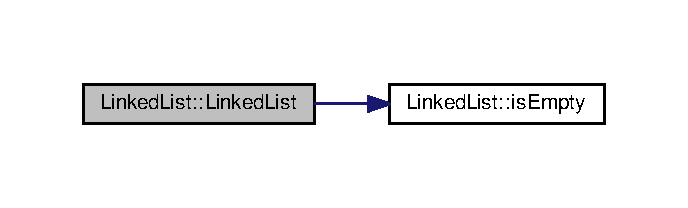
\includegraphics[width=330pt]{classLinkedList_a6d0ec2b365564af3f855d245a85bcbef_cgraph}
\end{center}
\end{figure}


\index{Linked\+List@{Linked\+List}!````~Linked\+List@{$\sim$\+Linked\+List}}
\index{````~Linked\+List@{$\sim$\+Linked\+List}!Linked\+List@{Linked\+List}}
\subsubsection[{\texorpdfstring{$\sim$\+Linked\+List()}{~LinkedList()}}]{\setlength{\rightskip}{0pt plus 5cm}template$<$class T $>$ {\bf Linked\+List}$<$ T $>$\+::$\sim${\bf Linked\+List} (
\begin{DoxyParamCaption}
{}
\end{DoxyParamCaption}
)}\hypertarget{classLinkedList_a7c37609df3b83bc4eb0281b852f93fd7}{}\label{classLinkedList_a7c37609df3b83bc4eb0281b852f93fd7}

\begin{DoxyCode}
41 \{
42    \hyperlink{classNode}{Node}* curr = \hyperlink{classLinkedList_a35e09287e2d2943707b011208e7a8ed2}{head};
43    \hyperlink{classNode}{Node}* del;
44    \textcolor{keywordflow}{while}(curr)
45    \{
46       del = curr;
47       curr = curr -> \hyperlink{classNode_af8f2d178f274dd254e6e1965971f0fd0}{getNext}();
48       \textcolor{keyword}{delete} del; \textcolor{comment}{//releases the Node memory                                                               
                                                                                                       }
49    \}
50    del = NULL;
51    \hyperlink{classLinkedList_a35e09287e2d2943707b011208e7a8ed2}{head} = NULL;
52 \}
\end{DoxyCode}


\subsection{Member Function Documentation}
\index{Linked\+List@{Linked\+List}!append@{append}}
\index{append@{append}!Linked\+List@{Linked\+List}}
\subsubsection[{\texorpdfstring{append(\+Node$<$ T $>$ $\ast$n)}{append(Node< T > *n)}}]{\setlength{\rightskip}{0pt plus 5cm}template$<$class T $>$ void {\bf Linked\+List}$<$ T $>$\+::append (
\begin{DoxyParamCaption}
\item[{{\bf Node}$<$ T $>$ $\ast$}]{n}
\end{DoxyParamCaption}
)\hspace{0.3cm}{\ttfamily [virtual]}}\hypertarget{classLinkedList_ac2f92598858e9ba02af8722fba803c53}{}\label{classLinkedList_ac2f92598858e9ba02af8722fba803c53}


Reimplemented in \hyperlink{classDoubleLinkedList_a5732ebaac8186c9847363c2569a1bf49}{Double\+Linked\+List$<$ T $>$}.


\begin{DoxyCode}
72 \{
73    \hyperlink{classNode}{Node}* curr;
74    \textcolor{keywordflow}{if}(\hyperlink{classLinkedList_a35e09287e2d2943707b011208e7a8ed2}{head} == NULL)
75       \hyperlink{classLinkedList_a35e09287e2d2943707b011208e7a8ed2}{head} = n; \textcolor{comment}{//first Node added to the list                                                         
                                                                                                           }
76    \textcolor{keywordflow}{else}
77    \{
78       curr = \hyperlink{classLinkedList_a35e09287e2d2943707b011208e7a8ed2}{head};
79       \textcolor{keywordflow}{while}(curr -> \hyperlink{classNode_af8f2d178f274dd254e6e1965971f0fd0}{getNext}() != NULL) \textcolor{comment}{//finds the last Node in the list                            
                                                                                                              }
80          curr = curr -> \hyperlink{classNode_af8f2d178f274dd254e6e1965971f0fd0}{getNext}();
81       curr -> \hyperlink{classNode_a0f69ba4f73cd616755f4ec0ae9fa7f96}{setNext}(n); \textcolor{comment}{//appends Node onto the end of the list                                   
                                                                                                              }
82    \}
83 \}
\end{DoxyCode}


Here is the call graph for this function\+:
\nopagebreak
\begin{figure}[H]
\begin{center}
\leavevmode
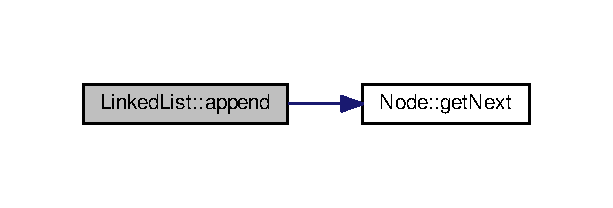
\includegraphics[width=294pt]{classLinkedList_ac2f92598858e9ba02af8722fba803c53_cgraph}
\end{center}
\end{figure}


\index{Linked\+List@{Linked\+List}!bubble\+Sort@{bubble\+Sort}}
\index{bubble\+Sort@{bubble\+Sort}!Linked\+List@{Linked\+List}}
\subsubsection[{\texorpdfstring{bubble\+Sort()}{bubbleSort()}}]{\setlength{\rightskip}{0pt plus 5cm}template$<$class T $>$ void {\bf Linked\+List}$<$ T $>$\+::bubble\+Sort (
\begin{DoxyParamCaption}
{}
\end{DoxyParamCaption}
)}\hypertarget{classLinkedList_aa644d66bfb879e71d1805a794a78b928}{}\label{classLinkedList_aa644d66bfb879e71d1805a794a78b928}

\begin{DoxyCode}
195 \{
196    \textcolor{keywordtype}{bool} sorted = \textcolor{keyword}{false};
197 
198    \textcolor{keywordflow}{if}(!\hyperlink{classLinkedList_a1b28b1e19e5aa68f3d89352e307928f6}{isEmpty}()) \textcolor{comment}{//checks if there are nodes in the list                                           
                                                                                                              }
199    \{
200       \textcolor{keywordflow}{for}(\textcolor{keywordtype}{int} k=0; k<\hyperlink{classLinkedList_ae04dbbcae32f8fb03dce3e174854981f}{getNumNode}()-1 && !sorted; k++)
201       \{
202          \hyperlink{classNode}{Node}* curr = \hyperlink{classLinkedList_a35e09287e2d2943707b011208e7a8ed2}{head}; \textcolor{comment}{//starts at beginning of the list                                      
                                                                                                               }
203          \textcolor{keywordtype}{int} currPos = 1;
204          \hyperlink{classNode}{Node}* nextNode = \hyperlink{classLinkedList_a35e09287e2d2943707b011208e7a8ed2}{head}->getNext(); \textcolor{comment}{//compares top node with second node                    
                                                                                                               }
205          \textcolor{keywordtype}{int} nextPos = 2;
206          sorted = \textcolor{keyword}{true}; \textcolor{comment}{//if sorted is true, that means the list is sorted and the loop will not continue
       checking                                                                                          }
207          \textcolor{keywordflow}{for}(\textcolor{keywordtype}{int} j=0; j < \hyperlink{classLinkedList_ae04dbbcae32f8fb03dce3e174854981f}{getNumNode}()-1-k; j++)
208          \{
209             \textcolor{keywordflow}{if}(curr->getStudent().getLastName().compare(nextNode->getStudent().getLastName()) < 0) \textcolor{comment}{//if the
       bottom student is higher in the alphabet}
210             \{
211                \hyperlink{classLinkedList_adea39e4b5d8f3fcb608c11f7746790ed}{swap}(curr, nextNode, currPos, nextPos); \textcolor{comment}{//swaps the two nodes                           
                                                                                                           }
212                sorted = \textcolor{keyword}{false};
213             \}
214             curr = curr->\hyperlink{classNode_af8f2d178f274dd254e6e1965971f0fd0}{getNext}(); \textcolor{comment}{//goes to next node                                             
                                                                                                              }
215             currPos++;
216             nextNode = nextNode->\hyperlink{classNode_af8f2d178f274dd254e6e1965971f0fd0}{getNext}();
217             nextPos++;
218          \}
219       \}
220    \}
221 \}
\end{DoxyCode}


Here is the call graph for this function\+:
\nopagebreak
\begin{figure}[H]
\begin{center}
\leavevmode
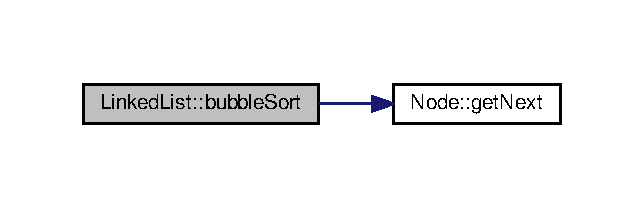
\includegraphics[width=309pt]{classLinkedList_aa644d66bfb879e71d1805a794a78b928_cgraph}
\end{center}
\end{figure}


\index{Linked\+List@{Linked\+List}!delete\+At\+Pos@{delete\+At\+Pos}}
\index{delete\+At\+Pos@{delete\+At\+Pos}!Linked\+List@{Linked\+List}}
\subsubsection[{\texorpdfstring{delete\+At\+Pos(int pos)}{deleteAtPos(int pos)}}]{\setlength{\rightskip}{0pt plus 5cm}template$<$class T $>$ void {\bf Linked\+List}$<$ T $>$\+::delete\+At\+Pos (
\begin{DoxyParamCaption}
\item[{int}]{pos}
\end{DoxyParamCaption}
)\hspace{0.3cm}{\ttfamily [virtual]}}\hypertarget{classLinkedList_a62a89a30509d38b88c75177b8efa9a98}{}\label{classLinkedList_a62a89a30509d38b88c75177b8efa9a98}


Reimplemented in \hyperlink{classDoubleLinkedList_a13520ddb52ec28efe42b5c29e9ba27e0}{Double\+Linked\+List$<$ T $>$}.


\begin{DoxyCode}
107 \{
108    \hyperlink{classNode}{Node}* curr = \hyperlink{classLinkedList_a35e09287e2d2943707b011208e7a8ed2}{head};
109    \hyperlink{classNode}{Node}* \hyperlink{classNode_ac953360c5f7ffae6ad13762189d34d9c}{prev} = NULL; \textcolor{comment}{//prev starts at NULL because curr starts at head                            
                                                                                                               }
110    \textcolor{keywordflow}{if}(pos <= \hyperlink{classLinkedList_ae04dbbcae32f8fb03dce3e174854981f}{getNumNode}() && pos > 0) \textcolor{comment}{//if position is in list parameters and the list is not
       empty                                                                                                         }
111    \{
112       \textcolor{keywordflow}{if}(pos == 1) \textcolor{comment}{//node is at the beginning of the list                                                  
                                                                                                       }
113          \hyperlink{classLinkedList_a35e09287e2d2943707b011208e7a8ed2}{head} = curr->\hyperlink{classNode_af8f2d178f274dd254e6e1965971f0fd0}{getNext}(); \textcolor{comment}{//takes node out of list                                       
                                                                                                                  }
114       \textcolor{keywordflow}{else} \textcolor{comment}{//node is in the middle of the list or at the end                                               
                                                                                                       }
115       \{
116          \textcolor{keywordflow}{for}(\textcolor{keywordtype}{int} k=1; k<pos; k++) \textcolor{comment}{//loop to arrive at the position                                         
                                                                                                       }
117          \{
118             prev = curr; \textcolor{comment}{//goes to next node                                                               
                                                                                                       }
119             curr = curr->\hyperlink{classNode_af8f2d178f274dd254e6e1965971f0fd0}{getNext}();
120          \}
121          prev->\hyperlink{classNode_a0f69ba4f73cd616755f4ec0ae9fa7f96}{setNext}(curr->\hyperlink{classNode_af8f2d178f274dd254e6e1965971f0fd0}{getNext}()); \textcolor{comment}{//takes node out of the list                        
                                                                                                                  
         }
122       \}
123       \textcolor{keyword}{delete} curr; \textcolor{comment}{//deletes node                                                                          
                                                                                                       }
124       curr = NULL;
125    \}
126 \}
\end{DoxyCode}


Here is the call graph for this function\+:
\nopagebreak
\begin{figure}[H]
\begin{center}
\leavevmode
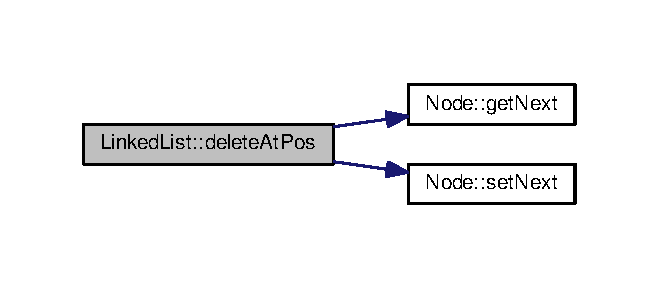
\includegraphics[width=316pt]{classLinkedList_a62a89a30509d38b88c75177b8efa9a98_cgraph}
\end{center}
\end{figure}


\index{Linked\+List@{Linked\+List}!display@{display}}
\index{display@{display}!Linked\+List@{Linked\+List}}
\subsubsection[{\texorpdfstring{display() const }{display() const }}]{\setlength{\rightskip}{0pt plus 5cm}template$<$class T $>$ void {\bf Linked\+List}$<$ T $>$\+::display (
\begin{DoxyParamCaption}
{}
\end{DoxyParamCaption}
) const}\hypertarget{classLinkedList_afddb5dbcc39e687add40de41b975cd8d}{}\label{classLinkedList_afddb5dbcc39e687add40de41b975cd8d}

\begin{DoxyCode}
129 \{
130    \hyperlink{classLinkedList_a7ed3bb4986b76cbfd3547d0b262ffff3}{displayNode}(\hyperlink{classLinkedList_a35e09287e2d2943707b011208e7a8ed2}{head});
131 \}
\end{DoxyCode}
\index{Linked\+List@{Linked\+List}!display\+Node@{display\+Node}}
\index{display\+Node@{display\+Node}!Linked\+List@{Linked\+List}}
\subsubsection[{\texorpdfstring{display\+Node(\+Node$<$ T $>$ $\ast$curr) const }{displayNode(Node< T > *curr) const }}]{\setlength{\rightskip}{0pt plus 5cm}template$<$class T $>$ void {\bf Linked\+List}$<$ T $>$\+::display\+Node (
\begin{DoxyParamCaption}
\item[{{\bf Node}$<$ T $>$ $\ast$}]{curr}
\end{DoxyParamCaption}
) const}\hypertarget{classLinkedList_a7ed3bb4986b76cbfd3547d0b262ffff3}{}\label{classLinkedList_a7ed3bb4986b76cbfd3547d0b262ffff3}

\begin{DoxyCode}
134 \{
135    \textcolor{keywordflow}{if}(curr) \textcolor{comment}{//checks to see if curr is not NULL                                                            
                                                                                                       }
136    \{
137       cout << curr -> getStudent() << endl; \textcolor{comment}{//displays Student information                                 
                                                                                                       }
138       \hyperlink{classLinkedList_a7ed3bb4986b76cbfd3547d0b262ffff3}{displayNode}(curr -> \hyperlink{classNode_af8f2d178f274dd254e6e1965971f0fd0}{getNext}()); \textcolor{comment}{//calls display with the next Node in the list     
                                                                                                                  
             }
139    \}
140 \}
\end{DoxyCode}
\index{Linked\+List@{Linked\+List}!get\+Head@{get\+Head}}
\index{get\+Head@{get\+Head}!Linked\+List@{Linked\+List}}
\subsubsection[{\texorpdfstring{get\+Head() const }{getHead() const }}]{\setlength{\rightskip}{0pt plus 5cm}template$<$class T $>$ {\bf Node}$<$ T $>$ $\ast$ {\bf Linked\+List}$<$ T $>$\+::get\+Head (
\begin{DoxyParamCaption}
{}
\end{DoxyParamCaption}
) const}\hypertarget{classLinkedList_af59e26b062e8e9549974adfa5bb51eb2}{}\label{classLinkedList_af59e26b062e8e9549974adfa5bb51eb2}

\begin{DoxyCode}
67 \{
68    \textcolor{keywordflow}{return} \hyperlink{classLinkedList_a35e09287e2d2943707b011208e7a8ed2}{head};
69 \}
\end{DoxyCode}
\index{Linked\+List@{Linked\+List}!get\+Num\+Node@{get\+Num\+Node}}
\index{get\+Num\+Node@{get\+Num\+Node}!Linked\+List@{Linked\+List}}
\subsubsection[{\texorpdfstring{get\+Num\+Node() const }{getNumNode() const }}]{\setlength{\rightskip}{0pt plus 5cm}template$<$class T $>$ int {\bf Linked\+List}$<$ T $>$\+::get\+Num\+Node (
\begin{DoxyParamCaption}
{}
\end{DoxyParamCaption}
) const}\hypertarget{classLinkedList_ae04dbbcae32f8fb03dce3e174854981f}{}\label{classLinkedList_ae04dbbcae32f8fb03dce3e174854981f}

\begin{DoxyCode}
55 \{
56    \hyperlink{classNode}{Node}* curr = \hyperlink{classLinkedList_a35e09287e2d2943707b011208e7a8ed2}{head};
57    \textcolor{keywordtype}{int} count = 0;
58    \textcolor{keywordflow}{while}(curr)
59    \{
60      count++; \textcolor{comment}{//adds to count for every Node in the list                                                   
                                                                                                      }
61       curr = curr -> \hyperlink{classNode_af8f2d178f274dd254e6e1965971f0fd0}{getNext}();
62    \}
63    \textcolor{keywordflow}{return} count;
64 \}
\end{DoxyCode}
\index{Linked\+List@{Linked\+List}!insert@{insert}}
\index{insert@{insert}!Linked\+List@{Linked\+List}}
\subsubsection[{\texorpdfstring{insert(\+Node$<$ T $>$ $\ast$n)}{insert(Node< T > *n)}}]{\setlength{\rightskip}{0pt plus 5cm}template$<$class T $>$ void {\bf Linked\+List}$<$ T $>$\+::insert (
\begin{DoxyParamCaption}
\item[{{\bf Node}$<$ T $>$ $\ast$}]{n}
\end{DoxyParamCaption}
)}\hypertarget{classLinkedList_a718246359a2199be67212703be951071}{}\label{classLinkedList_a718246359a2199be67212703be951071}

\begin{DoxyCode}
151 \{
152    \textcolor{keywordtype}{bool} foundPos = \textcolor{keyword}{false};
153    \hyperlink{classNode}{Node}* curr = \hyperlink{classLinkedList_a35e09287e2d2943707b011208e7a8ed2}{head};
154    \textcolor{keywordtype}{int} pos = 1;
155    \textcolor{keywordflow}{while}(curr && !foundPos) \textcolor{comment}{//finds the last Node in the list                                              
                                                                                                       }
156    \{
157       \textcolor{keywordflow}{if}(n->getStudent().getLastName().compare(curr->getStudent().getLastName()) > 0) \textcolor{comment}{//student's last name
       is father down in the alphabet                                                                  }
158       \{
159          curr = curr->\hyperlink{classNode_af8f2d178f274dd254e6e1965971f0fd0}{getNext}(); \textcolor{comment}{//go to next node                                                  
                                                                                                              }
160          pos++;
161       \}
162       \textcolor{keywordflow}{else} \textcolor{comment}{//student is at the right place alphabetically                                                  
                                                                                                       }
163       \{
164          \hyperlink{classLinkedList_aa7b12c5f9bb22be91012d68c9da0b431}{insertAtPos}(n, pos); \textcolor{comment}{//insert node at that position                                    
                                                                                                                  }
165          foundPos = \textcolor{keyword}{true};
166       \}
167    \}
168    \textcolor{keywordflow}{if}(!foundPos) \textcolor{comment}{//student is last in list alphabetically                                                  
                                                                                                       }
169       \hyperlink{classLinkedList_ac2f92598858e9ba02af8722fba803c53}{append}(n); \textcolor{comment}{//add to end of list                                                                
                                                                                                             }
170 \}
\end{DoxyCode}


Here is the call graph for this function\+:
\nopagebreak
\begin{figure}[H]
\begin{center}
\leavevmode
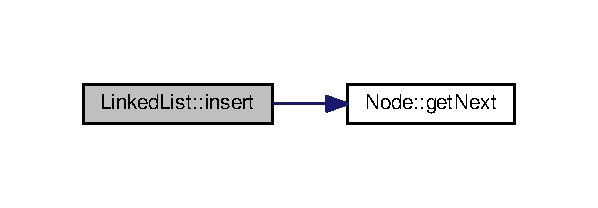
\includegraphics[width=287pt]{classLinkedList_a718246359a2199be67212703be951071_cgraph}
\end{center}
\end{figure}


\index{Linked\+List@{Linked\+List}!insert\+At\+Pos@{insert\+At\+Pos}}
\index{insert\+At\+Pos@{insert\+At\+Pos}!Linked\+List@{Linked\+List}}
\subsubsection[{\texorpdfstring{insert\+At\+Pos(\+Node$<$ T $>$ $\ast$n, int pos)}{insertAtPos(Node< T > *n, int pos)}}]{\setlength{\rightskip}{0pt plus 5cm}template$<$class T $>$ void {\bf Linked\+List}$<$ T $>$\+::insert\+At\+Pos (
\begin{DoxyParamCaption}
\item[{{\bf Node}$<$ T $>$ $\ast$}]{n, }
\item[{int}]{pos}
\end{DoxyParamCaption}
)\hspace{0.3cm}{\ttfamily [virtual]}}\hypertarget{classLinkedList_aa7b12c5f9bb22be91012d68c9da0b431}{}\label{classLinkedList_aa7b12c5f9bb22be91012d68c9da0b431}


Reimplemented in \hyperlink{classDoubleLinkedList_abd88472eeb1c4904b9e92d712e652d45}{Double\+Linked\+List$<$ T $>$}.


\begin{DoxyCode}
173 \{
174    \hyperlink{classNode}{Node}* before = NULL;
175    \hyperlink{classNode}{Node}* after = \hyperlink{classLinkedList_a35e09287e2d2943707b011208e7a8ed2}{head};
176    \textcolor{keywordflow}{if}(pos <= \hyperlink{classLinkedList_ae04dbbcae32f8fb03dce3e174854981f}{getNumNode}() && pos > 0) \textcolor{comment}{//if position is in list parameters and the list is not
       empty                                                                                                         }
177    \{
178       \textcolor{keywordflow}{if}(pos == 1) \textcolor{comment}{//if the node should be placed at the beginning of the list                             
                                                                                                       }
179          \hyperlink{classLinkedList_a35e09287e2d2943707b011208e7a8ed2}{head} = n; \textcolor{comment}{//insert node at beginning}
180       \textcolor{keywordflow}{else}
181       \{
182          \textcolor{keywordflow}{for}(\textcolor{keywordtype}{int} k=1; k<pos; k++) \textcolor{comment}{//loop to arrive at the position requested                               
                                                                                                       }
183          \{
184             before = after;
185             after = after->\hyperlink{classNode_af8f2d178f274dd254e6e1965971f0fd0}{getNext}();
186          \}
187          before->\hyperlink{classNode_a0f69ba4f73cd616755f4ec0ae9fa7f96}{setNext}(n); \textcolor{comment}{//insert node                                                          
                                                                                                              }
188       \}
189       n->\hyperlink{classNode_a0f69ba4f73cd616755f4ec0ae9fa7f96}{setNext}(after);
190       after = NULL;
191    \}
192 \}
\end{DoxyCode}


Here is the call graph for this function\+:
\nopagebreak
\begin{figure}[H]
\begin{center}
\leavevmode
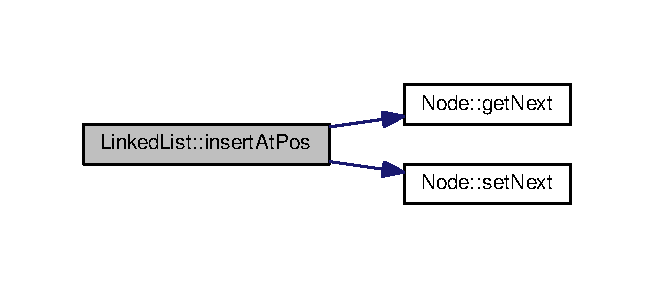
\includegraphics[width=314pt]{classLinkedList_aa7b12c5f9bb22be91012d68c9da0b431_cgraph}
\end{center}
\end{figure}


\index{Linked\+List@{Linked\+List}!is\+Empty@{is\+Empty}}
\index{is\+Empty@{is\+Empty}!Linked\+List@{Linked\+List}}
\subsubsection[{\texorpdfstring{is\+Empty() const }{isEmpty() const }}]{\setlength{\rightskip}{0pt plus 5cm}template$<$class T $>$ bool {\bf Linked\+List}$<$ T $>$\+::is\+Empty (
\begin{DoxyParamCaption}
{}
\end{DoxyParamCaption}
) const}\hypertarget{classLinkedList_a1b28b1e19e5aa68f3d89352e307928f6}{}\label{classLinkedList_a1b28b1e19e5aa68f3d89352e307928f6}

\begin{DoxyCode}
143 \{
144    \textcolor{keywordtype}{bool} empty = \textcolor{keyword}{false};
145    \textcolor{keywordflow}{if}(\hyperlink{classLinkedList_a35e09287e2d2943707b011208e7a8ed2}{head} == NULL) \textcolor{comment}{//is head is NULL, then there is no list of Nodes                                  
                                                                                                           }
146       empty = \textcolor{keyword}{true};
147    \textcolor{keywordflow}{return} empty;
148 \}
\end{DoxyCode}
\index{Linked\+List@{Linked\+List}!selection\+Sort@{selection\+Sort}}
\index{selection\+Sort@{selection\+Sort}!Linked\+List@{Linked\+List}}
\subsubsection[{\texorpdfstring{selection\+Sort()}{selectionSort()}}]{\setlength{\rightskip}{0pt plus 5cm}template$<$class T $>$ void {\bf Linked\+List}$<$ T $>$\+::selection\+Sort (
\begin{DoxyParamCaption}
{}
\end{DoxyParamCaption}
)}\hypertarget{classLinkedList_abd329a83adcec046dc482f7566cf91f4}{}\label{classLinkedList_abd329a83adcec046dc482f7566cf91f4}

\begin{DoxyCode}
224 \{
225    \textcolor{keywordflow}{if}(!\hyperlink{classLinkedList_a1b28b1e19e5aa68f3d89352e307928f6}{isEmpty}()) \textcolor{comment}{//checks if there are nodes in the list                                           
                                                                                                              }
226    \{
227       \textcolor{keywordflow}{for}(\textcolor{keywordtype}{int} k=\hyperlink{classLinkedList_ae04dbbcae32f8fb03dce3e174854981f}{getNumNode}()-1; k>=0; k--)
228       \{
229          \hyperlink{classNode}{Node}* curr = \hyperlink{classLinkedList_a35e09287e2d2943707b011208e7a8ed2}{head};
230          \hyperlink{classNode}{Node}* largest = curr; \textcolor{comment}{//student with name farthest in the alphabet. Default start at head     
                                                                                                           }
231          \textcolor{keywordtype}{int} currPos = 1;
232          \textcolor{keywordtype}{int} largestPos = currPos; \textcolor{comment}{//position of the largest node is defaulted to the first node in the
       list                                                                                                }
233          \textcolor{keywordflow}{for}(\textcolor{keywordtype}{int} j=0; j<=k; j++)
234          \{
235             \textcolor{keywordflow}{if}(curr->getStudent().getLastName().compare(largest->getStudent().getLastName()) > 0) \textcolor{comment}{//if the
       student is farther down in the alphabet than the largest                                         }
236             \{
237                largest = curr; \textcolor{comment}{//that student is the new largest                                           
                                                                                                       }
238                largestPos = currPos;
239             \}
240             \textcolor{keywordflow}{if}(currPos <= k) \textcolor{comment}{//moves to net node only if currPos is less than or equal to k                
                                                                                                       }
241             \{
242                curr = curr->\hyperlink{classNode_af8f2d178f274dd254e6e1965971f0fd0}{getNext}(); \textcolor{comment}{//go to the next node                                        
                                                                                                              }
243                currPos++;
244             \}
245          \}
246          \textcolor{keywordflow}{if}((largestPos != currPos) && (currPos != 1)) \textcolor{comment}{//if the largest node is not the last node          
                                                                                                       }
247             \hyperlink{classLinkedList_adea39e4b5d8f3fcb608c11f7746790ed}{swap}(largest, curr, largestPos, currPos); \textcolor{comment}{//swaps the largest node with the last node      
                                                                                                           }
248       \}
249    \}
250 \}
\end{DoxyCode}


Here is the call graph for this function\+:
\nopagebreak
\begin{figure}[H]
\begin{center}
\leavevmode
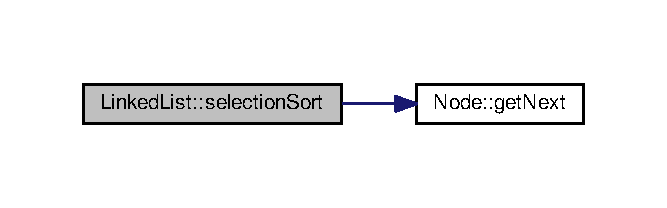
\includegraphics[width=320pt]{classLinkedList_abd329a83adcec046dc482f7566cf91f4_cgraph}
\end{center}
\end{figure}


\index{Linked\+List@{Linked\+List}!swap@{swap}}
\index{swap@{swap}!Linked\+List@{Linked\+List}}
\subsubsection[{\texorpdfstring{swap(\+Node$<$ T $>$ $\ast$\&f, Node$<$ T $>$ $\ast$\&l, int f\+Pos, int l\+Pos)}{swap(Node< T > *&f, Node< T > *&l, int fPos, int lPos)}}]{\setlength{\rightskip}{0pt plus 5cm}template$<$class T $>$ void {\bf Linked\+List}$<$ T $>$\+::swap (
\begin{DoxyParamCaption}
\item[{{\bf Node}$<$ T $>$ $\ast$\&}]{f, }
\item[{{\bf Node}$<$ T $>$ $\ast$\&}]{l, }
\item[{int}]{f\+Pos, }
\item[{int}]{l\+Pos}
\end{DoxyParamCaption}
)}\hypertarget{classLinkedList_adea39e4b5d8f3fcb608c11f7746790ed}{}\label{classLinkedList_adea39e4b5d8f3fcb608c11f7746790ed}

\begin{DoxyCode}
253 \{
254    \hyperlink{classNode}{Node}* fTemp = \textcolor{keyword}{new} \hyperlink{classNode_a0ac1d44cfe588be564acf25485029bd8}{Node}(*f); \textcolor{comment}{//create new nodes that are identical to the ones being swapped     
                                                                                                               }
255    \hyperlink{classNode}{Node}* lTemp = \textcolor{keyword}{new} \hyperlink{classNode_a0ac1d44cfe588be564acf25485029bd8}{Node}(*l);
256 
257    \hyperlink{classLinkedList_a62a89a30509d38b88c75177b8efa9a98}{deleteAtPos}(fPos); \textcolor{comment}{//deletes first of the two nodes                                          
                                                                                                                  }
258    \hyperlink{classLinkedList_aa7b12c5f9bb22be91012d68c9da0b431}{insertAtPos}(lTemp, fPos); \textcolor{comment}{//places copied node in that position                              
                                                                                                                  }
259    \hyperlink{classLinkedList_a62a89a30509d38b88c75177b8efa9a98}{deleteAtPos}(lPos); \textcolor{comment}{//deletes second node                                                     
                                                                                                                  }
260    \textcolor{keywordflow}{if}(lPos > \hyperlink{classLinkedList_ae04dbbcae32f8fb03dce3e174854981f}{getNumNode}()) \textcolor{comment}{//if one of the nodes was the last node in the list, append the node  
                                                                                                                 }
261       \hyperlink{classLinkedList_ac2f92598858e9ba02af8722fba803c53}{append}(fTemp);
262    \textcolor{keywordflow}{else}
263       \hyperlink{classLinkedList_aa7b12c5f9bb22be91012d68c9da0b431}{insertAtPos}(fTemp, lPos); \textcolor{comment}{//insert node at the position in the list                       
                                                                                                                  }
264 
265    f = lTemp; \textcolor{comment}{//swap the pointers that were passed by reference                                            
                                                                                                       }
266    l = fTemp;
267 \}
\end{DoxyCode}


\subsection{Member Data Documentation}
\index{Linked\+List@{Linked\+List}!head@{head}}
\index{head@{head}!Linked\+List@{Linked\+List}}
\subsubsection[{\texorpdfstring{head}{head}}]{\setlength{\rightskip}{0pt plus 5cm}template$<$class T$>$ {\bf Node}$<$T$>$$\ast$ {\bf Linked\+List}$<$ T $>$\+::head\hspace{0.3cm}{\ttfamily [protected]}}\hypertarget{classLinkedList_a35e09287e2d2943707b011208e7a8ed2}{}\label{classLinkedList_a35e09287e2d2943707b011208e7a8ed2}


The documentation for this class was generated from the following files\+:\begin{DoxyCompactItemize}
\item 
\hyperlink{LinkedList_8h}{Linked\+List.\+h}\item 
\hyperlink{LinkedList_8cpp}{Linked\+List.\+cpp}\end{DoxyCompactItemize}

\hypertarget{classNode}{}\section{Node Class Reference}
\label{classNode}\index{Node@{Node}}


{\ttfamily \#include $<$Calculo\+Tempo\+\_\+node.\+h$>$}



Collaboration diagram for Node\+:
\nopagebreak
\begin{figure}[H]
\begin{center}
\leavevmode
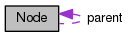
\includegraphics[width=169pt]{classNode__coll__graph}
\end{center}
\end{figure}
\subsection*{Public Member Functions}
\begin{DoxyCompactItemize}
\item 
\hyperlink{classNode_ad7a34779cad45d997bfd6d3d8043c75f}{Node} ()
\item 
\hyperlink{classNode_a2d13f7f1172705cddb79039c2fabbba6}{Node} (int x, int y, \hyperlink{classNode}{Node} $\ast$\+\_\+parent=0, int t=0)
\item 
int \hyperlink{classNode_a81aba8cc7d7ebd60051bb7cba210f587}{getx\+Pos} () const 
\item 
int \hyperlink{classNode_a7d26325d2355b29184cd6b428a78508b}{gety\+Pos} () const 
\item 
float \hyperlink{classNode_ab72b743b5abe69381e9066f4225793d2}{getG} () const 
\item 
float \hyperlink{classNode_ae6f0fa0586f0bba0a33ec57323849d89}{getH} () const 
\item 
float \hyperlink{classNode_ad22eea937020953945d47dc25667baf3}{getF} () const 
\item 
\hyperlink{classNode}{Node} $\ast$ \hyperlink{classNode_aee7fa50380cd3d5fd82c022e45ba2d37}{get\+Parent} () const 
\item 
void \hyperlink{classNode_a95d9ff38e9706097f752df46e1c912d9}{setx\+Pos} (int)
\item 
void \hyperlink{classNode_afcef18b84545fc9097c67ba6b48f31cb}{sety\+Pos} (int)
\item 
void \hyperlink{classNode_ac269852dd9117461a6069589470c39f1}{setG} (float)
\item 
void \hyperlink{classNode_aa10f28d0b00917bc5106373c73eb636f}{setH} (\hyperlink{classNode}{Node} $\ast$meta)
\item 
void \hyperlink{classNode_a77ef44966d6056821545f6b8acee2031}{setF} (float)
\item 
void \hyperlink{classNode_aaed3b50ac429bae4e3460f19c23a9f71}{set\+Parent} (\hyperlink{classNode}{Node} $\ast$)
\item 
void \hyperlink{classNode_aedfbcdc45d98f312e507e34e18b26093}{calculaF} ()
\end{DoxyCompactItemize}
\subsection*{Public Attributes}
\begin{DoxyCompactItemize}
\item 
int \hyperlink{classNode_ab61bfe3b52ba63f10939bf88270321e0}{tamanho}
\item 
int \hyperlink{classNode_a59a543130a10c95f1e8642cf8c5645e8}{id}
\item 
\hyperlink{classNode}{Node} $\ast$ \hyperlink{classNode_ad8184598cdea70e4bbdfd76f2b0f9e85}{parent}
\end{DoxyCompactItemize}
\subsection*{Private Attributes}
\begin{DoxyCompactItemize}
\item 
int \hyperlink{classNode_a4c5b1e397eba5f462edc72d5c031b33e}{x\+Pos}
\item 
int \hyperlink{classNode_ace45ec1cc1cc78ef699918a7adeb1dad}{y\+Pos}
\item 
float \hyperlink{classNode_a3c6a67023068f762eaaa8a4861ab3e9f}{G}
\item 
float \hyperlink{classNode_a26426055f336a81dc05680b981e4c270}{H}
\item 
float \hyperlink{classNode_aa68bc86c2839aca9c05e43541dc973a5}{F}
\end{DoxyCompactItemize}


\subsection{Constructor \& Destructor Documentation}
\index{Node@{Node}!Node@{Node}}
\index{Node@{Node}!Node@{Node}}
\subsubsection[{\texorpdfstring{Node()}{Node()}}]{\setlength{\rightskip}{0pt plus 5cm}Node\+::\+Node (
\begin{DoxyParamCaption}
{}
\end{DoxyParamCaption}
)\hspace{0.3cm}{\ttfamily [inline]}}\hypertarget{classNode_ad7a34779cad45d997bfd6d3d8043c75f}{}\label{classNode_ad7a34779cad45d997bfd6d3d8043c75f}

\begin{DoxyCode}
19 : \hyperlink{classNode_ad8184598cdea70e4bbdfd76f2b0f9e85}{parent}(0) \{\}
\end{DoxyCode}
\index{Node@{Node}!Node@{Node}}
\index{Node@{Node}!Node@{Node}}
\subsubsection[{\texorpdfstring{Node(int x, int y, Node $\ast$\+\_\+parent=0, int t=0)}{Node(int x, int y, Node *_parent=0, int t=0)}}]{\setlength{\rightskip}{0pt plus 5cm}Node\+::\+Node (
\begin{DoxyParamCaption}
\item[{int}]{x, }
\item[{int}]{y, }
\item[{{\bf Node} $\ast$}]{\+\_\+parent = {\ttfamily 0}, }
\item[{int}]{t = {\ttfamily 0}}
\end{DoxyParamCaption}
)\hspace{0.3cm}{\ttfamily [inline]}}\hypertarget{classNode_a2d13f7f1172705cddb79039c2fabbba6}{}\label{classNode_a2d13f7f1172705cddb79039c2fabbba6}

\begin{DoxyCode}
22 : \hyperlink{classNode_a4c5b1e397eba5f462edc72d5c031b33e}{xPos}(x),\hyperlink{classNode_ace45ec1cc1cc78ef699918a7adeb1dad}{yPos}(y),\hyperlink{classNode_a3c6a67023068f762eaaa8a4861ab3e9f}{G}(0),\hyperlink{classNode_a26426055f336a81dc05680b981e4c270}{H}(0),\hyperlink{classNode_ab61bfe3b52ba63f10939bf88270321e0}{tamanho}(t),\hyperlink{classNode_a59a543130a10c95f1e8642cf8c5645e8}{id}(y*\hyperlink{classNode_ab61bfe3b52ba63f10939bf88270321e0}{tamanho}+x),
      \hyperlink{classNode_ad8184598cdea70e4bbdfd76f2b0f9e85}{parent}(\_parent)\{\};
\end{DoxyCode}


Here is the call graph for this function\+:
\nopagebreak
\begin{figure}[H]
\begin{center}
\leavevmode
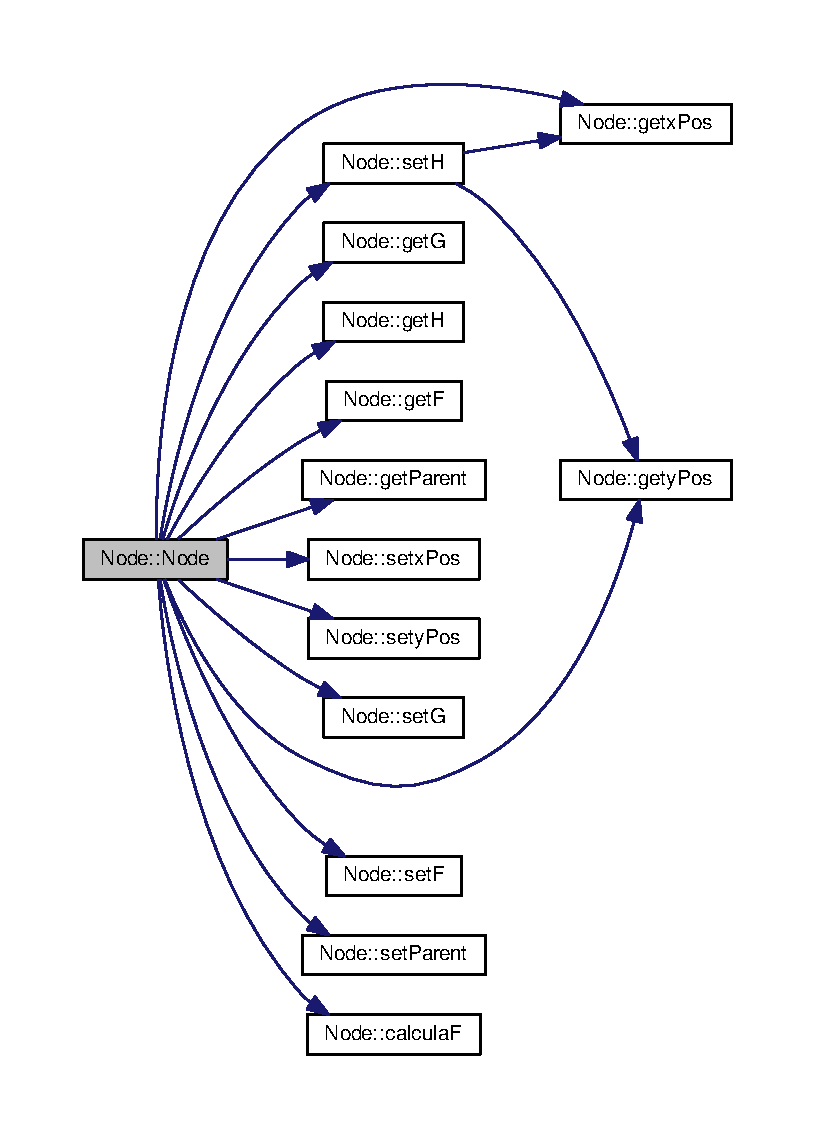
\includegraphics[width=350pt]{classNode_a2d13f7f1172705cddb79039c2fabbba6_cgraph}
\end{center}
\end{figure}




\subsection{Member Function Documentation}
\index{Node@{Node}!calculaF@{calculaF}}
\index{calculaF@{calculaF}!Node@{Node}}
\subsubsection[{\texorpdfstring{calcula\+F()}{calculaF()}}]{\setlength{\rightskip}{0pt plus 5cm}void Node\+::calculaF (
\begin{DoxyParamCaption}
{}
\end{DoxyParamCaption}
)}\hypertarget{classNode_aedfbcdc45d98f312e507e34e18b26093}{}\label{classNode_aedfbcdc45d98f312e507e34e18b26093}

\begin{DoxyCode}
109 \{
110     this->\hyperlink{classNode_aa68bc86c2839aca9c05e43541dc973a5}{F} = this->\hyperlink{classNode_a3c6a67023068f762eaaa8a4861ab3e9f}{G} + this->\hyperlink{classNode_a26426055f336a81dc05680b981e4c270}{H};
111 \}
\end{DoxyCode}
\index{Node@{Node}!getF@{getF}}
\index{getF@{getF}!Node@{Node}}
\subsubsection[{\texorpdfstring{get\+F() const }{getF() const }}]{\setlength{\rightskip}{0pt plus 5cm}float Node\+::getF (
\begin{DoxyParamCaption}
{}
\end{DoxyParamCaption}
) const}\hypertarget{classNode_ad22eea937020953945d47dc25667baf3}{}\label{classNode_ad22eea937020953945d47dc25667baf3}

\begin{DoxyCode}
76 \{
77     \textcolor{keywordflow}{return} this->\hyperlink{classNode_aa68bc86c2839aca9c05e43541dc973a5}{F};
78 \}
\end{DoxyCode}
\index{Node@{Node}!getG@{getG}}
\index{getG@{getG}!Node@{Node}}
\subsubsection[{\texorpdfstring{get\+G() const }{getG() const }}]{\setlength{\rightskip}{0pt plus 5cm}float Node\+::getG (
\begin{DoxyParamCaption}
{}
\end{DoxyParamCaption}
) const}\hypertarget{classNode_ab72b743b5abe69381e9066f4225793d2}{}\label{classNode_ab72b743b5abe69381e9066f4225793d2}

\begin{DoxyCode}
68 \{
69     \textcolor{keywordflow}{return} this->\hyperlink{classNode_a3c6a67023068f762eaaa8a4861ab3e9f}{G}; 
70 \}
\end{DoxyCode}
\index{Node@{Node}!getH@{getH}}
\index{getH@{getH}!Node@{Node}}
\subsubsection[{\texorpdfstring{get\+H() const }{getH() const }}]{\setlength{\rightskip}{0pt plus 5cm}float Node\+::getH (
\begin{DoxyParamCaption}
{}
\end{DoxyParamCaption}
) const}\hypertarget{classNode_ae6f0fa0586f0bba0a33ec57323849d89}{}\label{classNode_ae6f0fa0586f0bba0a33ec57323849d89}

\begin{DoxyCode}
72 \{
73     \textcolor{keywordflow}{return} this->\hyperlink{classNode_a26426055f336a81dc05680b981e4c270}{H};
74 \}
\end{DoxyCode}
\index{Node@{Node}!get\+Parent@{get\+Parent}}
\index{get\+Parent@{get\+Parent}!Node@{Node}}
\subsubsection[{\texorpdfstring{get\+Parent() const }{getParent() const }}]{\setlength{\rightskip}{0pt plus 5cm}{\bf Node} $\ast$ Node\+::get\+Parent (
\begin{DoxyParamCaption}
{}
\end{DoxyParamCaption}
) const}\hypertarget{classNode_aee7fa50380cd3d5fd82c022e45ba2d37}{}\label{classNode_aee7fa50380cd3d5fd82c022e45ba2d37}

\begin{DoxyCode}
80 \{
81     \textcolor{keywordflow}{return} this->\hyperlink{classNode_ad8184598cdea70e4bbdfd76f2b0f9e85}{parent};
82 \}
\end{DoxyCode}
\index{Node@{Node}!getx\+Pos@{getx\+Pos}}
\index{getx\+Pos@{getx\+Pos}!Node@{Node}}
\subsubsection[{\texorpdfstring{getx\+Pos() const }{getxPos() const }}]{\setlength{\rightskip}{0pt plus 5cm}int Node\+::getx\+Pos (
\begin{DoxyParamCaption}
{}
\end{DoxyParamCaption}
) const}\hypertarget{classNode_a81aba8cc7d7ebd60051bb7cba210f587}{}\label{classNode_a81aba8cc7d7ebd60051bb7cba210f587}

\begin{DoxyCode}
60 \{
61     \textcolor{keywordflow}{return} this->\hyperlink{classNode_a4c5b1e397eba5f462edc72d5c031b33e}{xPos};
62 \}
\end{DoxyCode}
\index{Node@{Node}!gety\+Pos@{gety\+Pos}}
\index{gety\+Pos@{gety\+Pos}!Node@{Node}}
\subsubsection[{\texorpdfstring{gety\+Pos() const }{getyPos() const }}]{\setlength{\rightskip}{0pt plus 5cm}int Node\+::gety\+Pos (
\begin{DoxyParamCaption}
{}
\end{DoxyParamCaption}
) const}\hypertarget{classNode_a7d26325d2355b29184cd6b428a78508b}{}\label{classNode_a7d26325d2355b29184cd6b428a78508b}

\begin{DoxyCode}
64 \{
65     \textcolor{keywordflow}{return} this->\hyperlink{classNode_ace45ec1cc1cc78ef699918a7adeb1dad}{yPos};
66 \}
\end{DoxyCode}
\index{Node@{Node}!setF@{setF}}
\index{setF@{setF}!Node@{Node}}
\subsubsection[{\texorpdfstring{set\+F(float)}{setF(float)}}]{\setlength{\rightskip}{0pt plus 5cm}void Node\+::setF (
\begin{DoxyParamCaption}
\item[{float}]{F}
\end{DoxyParamCaption}
)}\hypertarget{classNode_a77ef44966d6056821545f6b8acee2031}{}\label{classNode_a77ef44966d6056821545f6b8acee2031}

\begin{DoxyCode}
101 \{
102     this->\hyperlink{classNode_aa68bc86c2839aca9c05e43541dc973a5}{F} = \hyperlink{classNode_aa68bc86c2839aca9c05e43541dc973a5}{F};
103 \}
\end{DoxyCode}
\index{Node@{Node}!setG@{setG}}
\index{setG@{setG}!Node@{Node}}
\subsubsection[{\texorpdfstring{set\+G(float)}{setG(float)}}]{\setlength{\rightskip}{0pt plus 5cm}void Node\+::setG (
\begin{DoxyParamCaption}
\item[{float}]{G}
\end{DoxyParamCaption}
)}\hypertarget{classNode_ac269852dd9117461a6069589470c39f1}{}\label{classNode_ac269852dd9117461a6069589470c39f1}

\begin{DoxyCode}
93 \{
94     this->\hyperlink{classNode_a3c6a67023068f762eaaa8a4861ab3e9f}{G} = \hyperlink{classNode_a3c6a67023068f762eaaa8a4861ab3e9f}{G};
95 \}
\end{DoxyCode}
\index{Node@{Node}!setH@{setH}}
\index{setH@{setH}!Node@{Node}}
\subsubsection[{\texorpdfstring{set\+H(\+Node $\ast$meta)}{setH(Node *meta)}}]{\setlength{\rightskip}{0pt plus 5cm}void Node\+::setH (
\begin{DoxyParamCaption}
\item[{{\bf Node} $\ast$}]{meta}
\end{DoxyParamCaption}
)}\hypertarget{classNode_aa10f28d0b00917bc5106373c73eb636f}{}\label{classNode_aa10f28d0b00917bc5106373c73eb636f}

\begin{DoxyCode}
97 \{
98     this->\hyperlink{classNode_a26426055f336a81dc05680b981e4c270}{H} = (sqrt(((meta->\hyperlink{classNode_a81aba8cc7d7ebd60051bb7cba210f587}{getxPos}()-this->\hyperlink{classNode_a4c5b1e397eba5f462edc72d5c031b33e}{xPos})*(meta->\hyperlink{classNode_a81aba8cc7d7ebd60051bb7cba210f587}{getxPos}()-this->
      \hyperlink{classNode_a4c5b1e397eba5f462edc72d5c031b33e}{xPos}))+((meta->\hyperlink{classNode_a7d26325d2355b29184cd6b428a78508b}{getyPos}()-this->\hyperlink{classNode_ace45ec1cc1cc78ef699918a7adeb1dad}{yPos})*(meta->\hyperlink{classNode_a7d26325d2355b29184cd6b428a78508b}{getyPos}()-this->
      \hyperlink{classNode_ace45ec1cc1cc78ef699918a7adeb1dad}{yPos}))));
99 \}
\end{DoxyCode}


Here is the call graph for this function\+:
\nopagebreak
\begin{figure}[H]
\begin{center}
\leavevmode
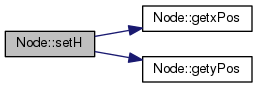
\includegraphics[width=265pt]{classNode_aa10f28d0b00917bc5106373c73eb636f_cgraph}
\end{center}
\end{figure}


\index{Node@{Node}!set\+Parent@{set\+Parent}}
\index{set\+Parent@{set\+Parent}!Node@{Node}}
\subsubsection[{\texorpdfstring{set\+Parent(\+Node $\ast$)}{setParent(Node *)}}]{\setlength{\rightskip}{0pt plus 5cm}void Node\+::set\+Parent (
\begin{DoxyParamCaption}
\item[{{\bf Node} $\ast$}]{parent}
\end{DoxyParamCaption}
)}\hypertarget{classNode_aaed3b50ac429bae4e3460f19c23a9f71}{}\label{classNode_aaed3b50ac429bae4e3460f19c23a9f71}

\begin{DoxyCode}
105 \{
106     this->parent = \hyperlink{classNode_ad8184598cdea70e4bbdfd76f2b0f9e85}{parent};
107 \}
\end{DoxyCode}
\index{Node@{Node}!setx\+Pos@{setx\+Pos}}
\index{setx\+Pos@{setx\+Pos}!Node@{Node}}
\subsubsection[{\texorpdfstring{setx\+Pos(int)}{setxPos(int)}}]{\setlength{\rightskip}{0pt plus 5cm}void Node\+::setx\+Pos (
\begin{DoxyParamCaption}
\item[{int}]{x}
\end{DoxyParamCaption}
)}\hypertarget{classNode_a95d9ff38e9706097f752df46e1c912d9}{}\label{classNode_a95d9ff38e9706097f752df46e1c912d9}

\begin{DoxyCode}
85 \{
86     this->\hyperlink{classNode_a4c5b1e397eba5f462edc72d5c031b33e}{xPos} = x;
87 \}
\end{DoxyCode}
\index{Node@{Node}!sety\+Pos@{sety\+Pos}}
\index{sety\+Pos@{sety\+Pos}!Node@{Node}}
\subsubsection[{\texorpdfstring{sety\+Pos(int)}{setyPos(int)}}]{\setlength{\rightskip}{0pt plus 5cm}void Node\+::sety\+Pos (
\begin{DoxyParamCaption}
\item[{int}]{y}
\end{DoxyParamCaption}
)}\hypertarget{classNode_afcef18b84545fc9097c67ba6b48f31cb}{}\label{classNode_afcef18b84545fc9097c67ba6b48f31cb}

\begin{DoxyCode}
89 \{
90     this->\hyperlink{classNode_ace45ec1cc1cc78ef699918a7adeb1dad}{yPos} = y;
91 \}
\end{DoxyCode}


\subsection{Member Data Documentation}
\index{Node@{Node}!F@{F}}
\index{F@{F}!Node@{Node}}
\subsubsection[{\texorpdfstring{F}{F}}]{\setlength{\rightskip}{0pt plus 5cm}float Node\+::F\hspace{0.3cm}{\ttfamily [private]}}\hypertarget{classNode_aa68bc86c2839aca9c05e43541dc973a5}{}\label{classNode_aa68bc86c2839aca9c05e43541dc973a5}
\index{Node@{Node}!G@{G}}
\index{G@{G}!Node@{Node}}
\subsubsection[{\texorpdfstring{G}{G}}]{\setlength{\rightskip}{0pt plus 5cm}float Node\+::G\hspace{0.3cm}{\ttfamily [private]}}\hypertarget{classNode_a3c6a67023068f762eaaa8a4861ab3e9f}{}\label{classNode_a3c6a67023068f762eaaa8a4861ab3e9f}
\index{Node@{Node}!H@{H}}
\index{H@{H}!Node@{Node}}
\subsubsection[{\texorpdfstring{H}{H}}]{\setlength{\rightskip}{0pt plus 5cm}float Node\+::H\hspace{0.3cm}{\ttfamily [private]}}\hypertarget{classNode_a26426055f336a81dc05680b981e4c270}{}\label{classNode_a26426055f336a81dc05680b981e4c270}
\index{Node@{Node}!id@{id}}
\index{id@{id}!Node@{Node}}
\subsubsection[{\texorpdfstring{id}{id}}]{\setlength{\rightskip}{0pt plus 5cm}int Node\+::id}\hypertarget{classNode_a59a543130a10c95f1e8642cf8c5645e8}{}\label{classNode_a59a543130a10c95f1e8642cf8c5645e8}
\index{Node@{Node}!parent@{parent}}
\index{parent@{parent}!Node@{Node}}
\subsubsection[{\texorpdfstring{parent}{parent}}]{\setlength{\rightskip}{0pt plus 5cm}{\bf Node}$\ast$ Node\+::parent}\hypertarget{classNode_ad8184598cdea70e4bbdfd76f2b0f9e85}{}\label{classNode_ad8184598cdea70e4bbdfd76f2b0f9e85}
\index{Node@{Node}!tamanho@{tamanho}}
\index{tamanho@{tamanho}!Node@{Node}}
\subsubsection[{\texorpdfstring{tamanho}{tamanho}}]{\setlength{\rightskip}{0pt plus 5cm}int Node\+::tamanho}\hypertarget{classNode_ab61bfe3b52ba63f10939bf88270321e0}{}\label{classNode_ab61bfe3b52ba63f10939bf88270321e0}
\index{Node@{Node}!x\+Pos@{x\+Pos}}
\index{x\+Pos@{x\+Pos}!Node@{Node}}
\subsubsection[{\texorpdfstring{x\+Pos}{xPos}}]{\setlength{\rightskip}{0pt plus 5cm}int Node\+::x\+Pos\hspace{0.3cm}{\ttfamily [private]}}\hypertarget{classNode_a4c5b1e397eba5f462edc72d5c031b33e}{}\label{classNode_a4c5b1e397eba5f462edc72d5c031b33e}
\index{Node@{Node}!y\+Pos@{y\+Pos}}
\index{y\+Pos@{y\+Pos}!Node@{Node}}
\subsubsection[{\texorpdfstring{y\+Pos}{yPos}}]{\setlength{\rightskip}{0pt plus 5cm}int Node\+::y\+Pos\hspace{0.3cm}{\ttfamily [private]}}\hypertarget{classNode_ace45ec1cc1cc78ef699918a7adeb1dad}{}\label{classNode_ace45ec1cc1cc78ef699918a7adeb1dad}


The documentation for this class was generated from the following files\+:\begin{DoxyCompactItemize}
\item 
\hyperlink{CalculoTempo__node_8h}{Calculo\+Tempo\+\_\+node.\+h}\item 
\hyperlink{CalculoTempo__node_8cpp}{Calculo\+Tempo\+\_\+node.\+cpp}\end{DoxyCompactItemize}

\hypertarget{classStudent}{}\section{Student Class Reference}
\label{classStudent}\index{Student@{Student}}


{\ttfamily \#include $<$Student.\+h$>$}

\subsection*{Public Member Functions}
\begin{DoxyCompactItemize}
\item 
\hyperlink{classStudent_af9168cedbfa5565cf0b20c1a9d3f5c9d}{Student} ()
\item 
\hyperlink{classStudent_a557917f9af87042e5fa25bd7b1aeaa30}{Student} (string f, string l, char m, int s, int a)
\item 
\hyperlink{classStudent_a9b3d40ac356f6794eeae74ce473a5617}{Student} (const \hyperlink{classStudent}{Student} \&s)
\item 
void \hyperlink{classStudent_a30731c688a4d7e3c047605de86c78007}{set\+Name} (string f, string l, char m)
\item 
void \hyperlink{classStudent_a46dafabdf7259d22c2ed038d187018d6}{set\+S\+SN} (int s)
\item 
void \hyperlink{classStudent_aae26ec99b719c86b60b33e19bc4f3986}{set\+Age} (int a)
\item 
string \hyperlink{classStudent_ac0c4ea968202c325e11b33ef38087701}{get\+First\+Name} () const 
\item 
string \hyperlink{classStudent_ae58e20cf8d78eecdbbd34c04f7a2c846}{get\+Last\+Name} () const 
\item 
char \hyperlink{classStudent_a9f266c04ecea344e544f9e772921d17c}{get\+Middle\+Initial} () const 
\item 
int \hyperlink{classStudent_acb222ca39f470aaa1562a25d329e8378}{get\+S\+SN} () const 
\item 
int \hyperlink{classStudent_a05e941545afe646579a8e91dfc8f1953}{get\+Age} () const 
\item 
void \hyperlink{classStudent_afeae2ddd8936ba4f37064a8d751f51eb}{read} (istream \&in)
\item 
void \hyperlink{classStudent_a17a6f00e4ec4637f77a50c2769e69721}{print} (ostream \&out)
\item 
bool \hyperlink{classStudent_a3f82e382259835b187fd92f2b15fcb42}{operator$>$} (const \hyperlink{classStudent}{Student} \&s) const 
\item 
bool \hyperlink{classStudent_a4add57e859306b4a543368201ca0922f}{operator$<$} (const \hyperlink{classStudent}{Student} \&s) const 
\end{DoxyCompactItemize}
\subsection*{Private Attributes}
\begin{DoxyCompactItemize}
\item 
string \hyperlink{classStudent_a333c7d227c87fdfa821d0232e21f9006}{fname}
\item 
string \hyperlink{classStudent_a6c934004d6a468a354916bcf0f998190}{lname}
\item 
char \hyperlink{classStudent_afd8d4557f2ac6bb7681c32e691248328}{mi}
\item 
int \hyperlink{classStudent_aa7181a8aac86888176481f901bee2cbd}{ssn}
\item 
int \hyperlink{classStudent_a552a431a43ffc545d180424597d51f97}{age}
\end{DoxyCompactItemize}
\subsection*{Friends}
\begin{DoxyCompactItemize}
\item 
class \hyperlink{classStudent_a6db9d28bd448a131448276ee03de1e6d}{Node}
\item 
ostream \& \hyperlink{classStudent_a8ed16acc8384ea29641694cb182ac764}{operator$<$$<$} (ostream \&outs, const \hyperlink{classStudent}{Student} \&s)
\item 
istream \& \hyperlink{classStudent_a2d76cee765e6e0d66e66a27d10fa0a68}{operator$>$$>$} (istream \&ins, \hyperlink{classStudent}{Student} \&s)
\end{DoxyCompactItemize}


\subsection{Constructor \& Destructor Documentation}
\index{Student@{Student}!Student@{Student}}
\index{Student@{Student}!Student@{Student}}
\subsubsection[{\texorpdfstring{Student()}{Student()}}]{\setlength{\rightskip}{0pt plus 5cm}Student\+::\+Student (
\begin{DoxyParamCaption}
{}
\end{DoxyParamCaption}
)\hspace{0.3cm}{\ttfamily [inline]}}\hypertarget{classStudent_af9168cedbfa5565cf0b20c1a9d3f5c9d}{}\label{classStudent_af9168cedbfa5565cf0b20c1a9d3f5c9d}

\begin{DoxyCode}
32 : \hyperlink{classStudent_a333c7d227c87fdfa821d0232e21f9006}{fname}(\textcolor{stringliteral}{""}), \hyperlink{classStudent_a6c934004d6a468a354916bcf0f998190}{lname}(\textcolor{stringliteral}{""}), \hyperlink{classStudent_afd8d4557f2ac6bb7681c32e691248328}{mi}(\textcolor{charliteral}{' '}), \hyperlink{classStudent_aa7181a8aac86888176481f901bee2cbd}{ssn}(0), \hyperlink{classStudent_a552a431a43ffc545d180424597d51f97}{age}(0) \{\} \textcolor{comment}{//default constructor                 
                                                                                                             }
\end{DoxyCode}
\index{Student@{Student}!Student@{Student}}
\index{Student@{Student}!Student@{Student}}
\subsubsection[{\texorpdfstring{Student(string f, string l, char m, int s, int a)}{Student(string f, string l, char m, int s, int a)}}]{\setlength{\rightskip}{0pt plus 5cm}Student\+::\+Student (
\begin{DoxyParamCaption}
\item[{string}]{f, }
\item[{string}]{l, }
\item[{char}]{m, }
\item[{int}]{s, }
\item[{int}]{a}
\end{DoxyParamCaption}
)\hspace{0.3cm}{\ttfamily [inline]}}\hypertarget{classStudent_a557917f9af87042e5fa25bd7b1aeaa30}{}\label{classStudent_a557917f9af87042e5fa25bd7b1aeaa30}

\begin{DoxyCode}
33 : \hyperlink{classStudent_a333c7d227c87fdfa821d0232e21f9006}{fname}(f), \hyperlink{classStudent_a6c934004d6a468a354916bcf0f998190}{lname}(l), \hyperlink{classStudent_afd8d4557f2ac6bb7681c32e691248328}{mi}(m), \hyperlink{classStudent_aa7181a8aac86888176481f901bee2cbd}{ssn}(s), \hyperlink{classStudent_a552a431a43ffc545d180424597d51f97}{age}(a) \{\}
\end{DoxyCode}
\index{Student@{Student}!Student@{Student}}
\index{Student@{Student}!Student@{Student}}
\subsubsection[{\texorpdfstring{Student(const Student \&s)}{Student(const Student &s)}}]{\setlength{\rightskip}{0pt plus 5cm}Student\+::\+Student (
\begin{DoxyParamCaption}
\item[{const {\bf Student} \&}]{s}
\end{DoxyParamCaption}
)}\hypertarget{classStudent_a9b3d40ac356f6794eeae74ce473a5617}{}\label{classStudent_a9b3d40ac356f6794eeae74ce473a5617}

\begin{DoxyCode}
14 \{
15    \hyperlink{classStudent_a333c7d227c87fdfa821d0232e21f9006}{fname} = s.\hyperlink{classStudent_a333c7d227c87fdfa821d0232e21f9006}{fname};
16    \hyperlink{classStudent_a6c934004d6a468a354916bcf0f998190}{lname} = s.\hyperlink{classStudent_a6c934004d6a468a354916bcf0f998190}{lname};
17    \hyperlink{classStudent_afd8d4557f2ac6bb7681c32e691248328}{mi} = s.\hyperlink{classStudent_afd8d4557f2ac6bb7681c32e691248328}{mi};
18    \hyperlink{classStudent_aa7181a8aac86888176481f901bee2cbd}{ssn} = s.\hyperlink{classStudent_aa7181a8aac86888176481f901bee2cbd}{ssn};
19    \hyperlink{classStudent_a552a431a43ffc545d180424597d51f97}{age} = s.\hyperlink{classStudent_a552a431a43ffc545d180424597d51f97}{age};
20 \}
\end{DoxyCode}


\subsection{Member Function Documentation}
\index{Student@{Student}!get\+Age@{get\+Age}}
\index{get\+Age@{get\+Age}!Student@{Student}}
\subsubsection[{\texorpdfstring{get\+Age() const }{getAge() const }}]{\setlength{\rightskip}{0pt plus 5cm}int Student\+::get\+Age (
\begin{DoxyParamCaption}
{}
\end{DoxyParamCaption}
) const}\hypertarget{classStudent_a05e941545afe646579a8e91dfc8f1953}{}\label{classStudent_a05e941545afe646579a8e91dfc8f1953}

\begin{DoxyCode}
60 \{
61    \textcolor{keywordflow}{return} \hyperlink{classStudent_a552a431a43ffc545d180424597d51f97}{age};
62 \}
\end{DoxyCode}
\index{Student@{Student}!get\+First\+Name@{get\+First\+Name}}
\index{get\+First\+Name@{get\+First\+Name}!Student@{Student}}
\subsubsection[{\texorpdfstring{get\+First\+Name() const }{getFirstName() const }}]{\setlength{\rightskip}{0pt plus 5cm}string Student\+::get\+First\+Name (
\begin{DoxyParamCaption}
{}
\end{DoxyParamCaption}
) const}\hypertarget{classStudent_ac0c4ea968202c325e11b33ef38087701}{}\label{classStudent_ac0c4ea968202c325e11b33ef38087701}

\begin{DoxyCode}
40 \{
41    \textcolor{keywordflow}{return} \hyperlink{classStudent_a333c7d227c87fdfa821d0232e21f9006}{fname};
42 \}
\end{DoxyCode}
\index{Student@{Student}!get\+Last\+Name@{get\+Last\+Name}}
\index{get\+Last\+Name@{get\+Last\+Name}!Student@{Student}}
\subsubsection[{\texorpdfstring{get\+Last\+Name() const }{getLastName() const }}]{\setlength{\rightskip}{0pt plus 5cm}string Student\+::get\+Last\+Name (
\begin{DoxyParamCaption}
{}
\end{DoxyParamCaption}
) const}\hypertarget{classStudent_ae58e20cf8d78eecdbbd34c04f7a2c846}{}\label{classStudent_ae58e20cf8d78eecdbbd34c04f7a2c846}

\begin{DoxyCode}
45 \{
46    \textcolor{keywordflow}{return} \hyperlink{classStudent_a6c934004d6a468a354916bcf0f998190}{lname};
47 \}
\end{DoxyCode}
\index{Student@{Student}!get\+Middle\+Initial@{get\+Middle\+Initial}}
\index{get\+Middle\+Initial@{get\+Middle\+Initial}!Student@{Student}}
\subsubsection[{\texorpdfstring{get\+Middle\+Initial() const }{getMiddleInitial() const }}]{\setlength{\rightskip}{0pt plus 5cm}char Student\+::get\+Middle\+Initial (
\begin{DoxyParamCaption}
{}
\end{DoxyParamCaption}
) const}\hypertarget{classStudent_a9f266c04ecea344e544f9e772921d17c}{}\label{classStudent_a9f266c04ecea344e544f9e772921d17c}

\begin{DoxyCode}
50 \{
51    \textcolor{keywordflow}{return} \hyperlink{classStudent_afd8d4557f2ac6bb7681c32e691248328}{mi};
52 \}
\end{DoxyCode}
\index{Student@{Student}!get\+S\+SN@{get\+S\+SN}}
\index{get\+S\+SN@{get\+S\+SN}!Student@{Student}}
\subsubsection[{\texorpdfstring{get\+S\+S\+N() const }{getSSN() const }}]{\setlength{\rightskip}{0pt plus 5cm}int Student\+::get\+S\+SN (
\begin{DoxyParamCaption}
{}
\end{DoxyParamCaption}
) const}\hypertarget{classStudent_acb222ca39f470aaa1562a25d329e8378}{}\label{classStudent_acb222ca39f470aaa1562a25d329e8378}

\begin{DoxyCode}
55 \{
56    \textcolor{keywordflow}{return} \hyperlink{classStudent_aa7181a8aac86888176481f901bee2cbd}{ssn};
57 \}
\end{DoxyCode}
\index{Student@{Student}!operator$<$@{operator$<$}}
\index{operator$<$@{operator$<$}!Student@{Student}}
\subsubsection[{\texorpdfstring{operator$<$(const Student \&s) const }{operator<(const Student &s) const }}]{\setlength{\rightskip}{0pt plus 5cm}bool Student\+::operator$<$ (
\begin{DoxyParamCaption}
\item[{const {\bf Student} \&}]{s}
\end{DoxyParamCaption}
) const}\hypertarget{classStudent_a4add57e859306b4a543368201ca0922f}{}\label{classStudent_a4add57e859306b4a543368201ca0922f}

\begin{DoxyCode}
94 \{
95    \textcolor{keywordflow}{return} (\hyperlink{classStudent_a6c934004d6a468a354916bcf0f998190}{lname}.compare(s.\hyperlink{classStudent_a6c934004d6a468a354916bcf0f998190}{lname}) < 0);
96 \}\end{DoxyCode}
\index{Student@{Student}!operator$>$@{operator$>$}}
\index{operator$>$@{operator$>$}!Student@{Student}}
\subsubsection[{\texorpdfstring{operator$>$(const Student \&s) const }{operator>(const Student &s) const }}]{\setlength{\rightskip}{0pt plus 5cm}bool Student\+::operator$>$ (
\begin{DoxyParamCaption}
\item[{const {\bf Student} \&}]{s}
\end{DoxyParamCaption}
) const}\hypertarget{classStudent_a3f82e382259835b187fd92f2b15fcb42}{}\label{classStudent_a3f82e382259835b187fd92f2b15fcb42}

\begin{DoxyCode}
89 \{
90    \textcolor{keywordflow}{return} (\hyperlink{classStudent_a6c934004d6a468a354916bcf0f998190}{lname}.compare(s.\hyperlink{classStudent_a6c934004d6a468a354916bcf0f998190}{lname}) > 0);
91 \}
\end{DoxyCode}
\index{Student@{Student}!print@{print}}
\index{print@{print}!Student@{Student}}
\subsubsection[{\texorpdfstring{print(ostream \&out)}{print(ostream &out)}}]{\setlength{\rightskip}{0pt plus 5cm}void Student\+::print (
\begin{DoxyParamCaption}
\item[{ostream \&}]{out}
\end{DoxyParamCaption}
)}\hypertarget{classStudent_a17a6f00e4ec4637f77a50c2769e69721}{}\label{classStudent_a17a6f00e4ec4637f77a50c2769e69721}

\begin{DoxyCode}
80 \{
81    out << \hyperlink{classStudent_a333c7d227c87fdfa821d0232e21f9006}{fname} << endl;
82    out << \hyperlink{classStudent_a6c934004d6a468a354916bcf0f998190}{lname} << endl;
83    out << \hyperlink{classStudent_afd8d4557f2ac6bb7681c32e691248328}{mi} << endl;
84    out << \hyperlink{classStudent_aa7181a8aac86888176481f901bee2cbd}{ssn} << endl;
85    out << \hyperlink{classStudent_a552a431a43ffc545d180424597d51f97}{age} << endl;
86 \}
\end{DoxyCode}
\index{Student@{Student}!read@{read}}
\index{read@{read}!Student@{Student}}
\subsubsection[{\texorpdfstring{read(istream \&in)}{read(istream &in)}}]{\setlength{\rightskip}{0pt plus 5cm}void Student\+::read (
\begin{DoxyParamCaption}
\item[{istream \&}]{in}
\end{DoxyParamCaption}
)}\hypertarget{classStudent_afeae2ddd8936ba4f37064a8d751f51eb}{}\label{classStudent_afeae2ddd8936ba4f37064a8d751f51eb}
\index{Student@{Student}!set\+Age@{set\+Age}}
\index{set\+Age@{set\+Age}!Student@{Student}}
\subsubsection[{\texorpdfstring{set\+Age(int a)}{setAge(int a)}}]{\setlength{\rightskip}{0pt plus 5cm}void Student\+::set\+Age (
\begin{DoxyParamCaption}
\item[{int}]{a}
\end{DoxyParamCaption}
)}\hypertarget{classStudent_aae26ec99b719c86b60b33e19bc4f3986}{}\label{classStudent_aae26ec99b719c86b60b33e19bc4f3986}

\begin{DoxyCode}
35 \{
36    \hyperlink{classStudent_a552a431a43ffc545d180424597d51f97}{age} = a;
37 \}
\end{DoxyCode}
\index{Student@{Student}!set\+Name@{set\+Name}}
\index{set\+Name@{set\+Name}!Student@{Student}}
\subsubsection[{\texorpdfstring{set\+Name(string f, string l, char m)}{setName(string f, string l, char m)}}]{\setlength{\rightskip}{0pt plus 5cm}void Student\+::set\+Name (
\begin{DoxyParamCaption}
\item[{string}]{f, }
\item[{string}]{l, }
\item[{char}]{m}
\end{DoxyParamCaption}
)}\hypertarget{classStudent_a30731c688a4d7e3c047605de86c78007}{}\label{classStudent_a30731c688a4d7e3c047605de86c78007}

\begin{DoxyCode}
23 \{
24    \hyperlink{classStudent_a333c7d227c87fdfa821d0232e21f9006}{fname} = f;
25    \hyperlink{classStudent_a6c934004d6a468a354916bcf0f998190}{lname} = l;
26    \hyperlink{classStudent_afd8d4557f2ac6bb7681c32e691248328}{mi} = m;
27 \}
\end{DoxyCode}
\index{Student@{Student}!set\+S\+SN@{set\+S\+SN}}
\index{set\+S\+SN@{set\+S\+SN}!Student@{Student}}
\subsubsection[{\texorpdfstring{set\+S\+S\+N(int s)}{setSSN(int s)}}]{\setlength{\rightskip}{0pt plus 5cm}void Student\+::set\+S\+SN (
\begin{DoxyParamCaption}
\item[{int}]{s}
\end{DoxyParamCaption}
)}\hypertarget{classStudent_a46dafabdf7259d22c2ed038d187018d6}{}\label{classStudent_a46dafabdf7259d22c2ed038d187018d6}

\begin{DoxyCode}
30 \{
31    \hyperlink{classStudent_aa7181a8aac86888176481f901bee2cbd}{ssn} = s;
32 \}
\end{DoxyCode}


\subsection{Friends And Related Function Documentation}
\index{Student@{Student}!Node@{Node}}
\index{Node@{Node}!Student@{Student}}
\subsubsection[{\texorpdfstring{Node}{Node}}]{\setlength{\rightskip}{0pt plus 5cm}friend class {\bf Node}\hspace{0.3cm}{\ttfamily [friend]}}\hypertarget{classStudent_a6db9d28bd448a131448276ee03de1e6d}{}\label{classStudent_a6db9d28bd448a131448276ee03de1e6d}
\index{Student@{Student}!operator$<$$<$@{operator$<$$<$}}
\index{operator$<$$<$@{operator$<$$<$}!Student@{Student}}
\subsubsection[{\texorpdfstring{operator$<$$<$}{operator<<}}]{\setlength{\rightskip}{0pt plus 5cm}ostream\& operator$<$$<$ (
\begin{DoxyParamCaption}
\item[{ostream \&}]{outs, }
\item[{const {\bf Student} \&}]{s}
\end{DoxyParamCaption}
)\hspace{0.3cm}{\ttfamily [friend]}}\hypertarget{classStudent_a8ed16acc8384ea29641694cb182ac764}{}\label{classStudent_a8ed16acc8384ea29641694cb182ac764}

\begin{DoxyCode}
65 \{
66    cout << \textcolor{stringliteral}{"Student:\(\backslash\)t\(\backslash\)t  "} << s.\hyperlink{classStudent_a6c934004d6a468a354916bcf0f998190}{lname} << \textcolor{stringliteral}{", "} << s.\hyperlink{classStudent_a333c7d227c87fdfa821d0232e21f9006}{fname} << \textcolor{stringliteral}{" "} << s.
      \hyperlink{classStudent_afd8d4557f2ac6bb7681c32e691248328}{mi} << endl;
67    cout << \textcolor{stringliteral}{"Social Security number:\(\backslash\)t  "} << s.\hyperlink{classStudent_aa7181a8aac86888176481f901bee2cbd}{ssn} << endl;
68    cout << \textcolor{stringliteral}{"Age:\(\backslash\)t\(\backslash\)t\(\backslash\)t  "} << s.\hyperlink{classStudent_a552a431a43ffc545d180424597d51f97}{age} << endl;
69    cout << \textcolor{stringliteral}{"------------------------------------------------------"} << endl;
70 
71    \textcolor{keywordflow}{return} outs;
72 \}
\end{DoxyCode}
\index{Student@{Student}!operator$>$$>$@{operator$>$$>$}}
\index{operator$>$$>$@{operator$>$$>$}!Student@{Student}}
\subsubsection[{\texorpdfstring{operator$>$$>$}{operator>>}}]{\setlength{\rightskip}{0pt plus 5cm}istream\& operator$>$$>$ (
\begin{DoxyParamCaption}
\item[{istream \&}]{ins, }
\item[{{\bf Student} \&}]{s}
\end{DoxyParamCaption}
)\hspace{0.3cm}{\ttfamily [friend]}}\hypertarget{classStudent_a2d76cee765e6e0d66e66a27d10fa0a68}{}\label{classStudent_a2d76cee765e6e0d66e66a27d10fa0a68}

\begin{DoxyCode}
75 \{
76    ins >> s.\hyperlink{classStudent_a333c7d227c87fdfa821d0232e21f9006}{fname} >> s.\hyperlink{classStudent_a6c934004d6a468a354916bcf0f998190}{lname} >> s.\hyperlink{classStudent_afd8d4557f2ac6bb7681c32e691248328}{mi} >> s.\hyperlink{classStudent_aa7181a8aac86888176481f901bee2cbd}{ssn} >> s.\hyperlink{classStudent_a552a431a43ffc545d180424597d51f97}{age};
77 \}
\end{DoxyCode}


\subsection{Member Data Documentation}
\index{Student@{Student}!age@{age}}
\index{age@{age}!Student@{Student}}
\subsubsection[{\texorpdfstring{age}{age}}]{\setlength{\rightskip}{0pt plus 5cm}int Student\+::age\hspace{0.3cm}{\ttfamily [private]}}\hypertarget{classStudent_a552a431a43ffc545d180424597d51f97}{}\label{classStudent_a552a431a43ffc545d180424597d51f97}
\index{Student@{Student}!fname@{fname}}
\index{fname@{fname}!Student@{Student}}
\subsubsection[{\texorpdfstring{fname}{fname}}]{\setlength{\rightskip}{0pt plus 5cm}string Student\+::fname\hspace{0.3cm}{\ttfamily [private]}}\hypertarget{classStudent_a333c7d227c87fdfa821d0232e21f9006}{}\label{classStudent_a333c7d227c87fdfa821d0232e21f9006}
\index{Student@{Student}!lname@{lname}}
\index{lname@{lname}!Student@{Student}}
\subsubsection[{\texorpdfstring{lname}{lname}}]{\setlength{\rightskip}{0pt plus 5cm}string Student\+::lname\hspace{0.3cm}{\ttfamily [private]}}\hypertarget{classStudent_a6c934004d6a468a354916bcf0f998190}{}\label{classStudent_a6c934004d6a468a354916bcf0f998190}
\index{Student@{Student}!mi@{mi}}
\index{mi@{mi}!Student@{Student}}
\subsubsection[{\texorpdfstring{mi}{mi}}]{\setlength{\rightskip}{0pt plus 5cm}char Student\+::mi\hspace{0.3cm}{\ttfamily [private]}}\hypertarget{classStudent_afd8d4557f2ac6bb7681c32e691248328}{}\label{classStudent_afd8d4557f2ac6bb7681c32e691248328}
\index{Student@{Student}!ssn@{ssn}}
\index{ssn@{ssn}!Student@{Student}}
\subsubsection[{\texorpdfstring{ssn}{ssn}}]{\setlength{\rightskip}{0pt plus 5cm}int Student\+::ssn\hspace{0.3cm}{\ttfamily [private]}}\hypertarget{classStudent_aa7181a8aac86888176481f901bee2cbd}{}\label{classStudent_aa7181a8aac86888176481f901bee2cbd}


The documentation for this class was generated from the following files\+:\begin{DoxyCompactItemize}
\item 
\hyperlink{Student_8h}{Student.\+h}\item 
\hyperlink{Student_8cpp}{Student.\+cpp}\end{DoxyCompactItemize}

\chapter{File Documentation}
\hypertarget{LinkedList_8cpp}{}\section{Linked\+List.\+cpp File Reference}
\label{LinkedList_8cpp}\index{Linked\+List.\+cpp@{Linked\+List.\+cpp}}
{\ttfamily \#include \char`\"{}Linked\+List.\+h\char`\"{}}\\*
{\ttfamily \#include \char`\"{}Node.\+h\char`\"{}}\\*
{\ttfamily \#include \char`\"{}Student.\+h\char`\"{}}\\*
Include dependency graph for Linked\+List.\+cpp\+:
\nopagebreak
\begin{figure}[H]
\begin{center}
\leavevmode
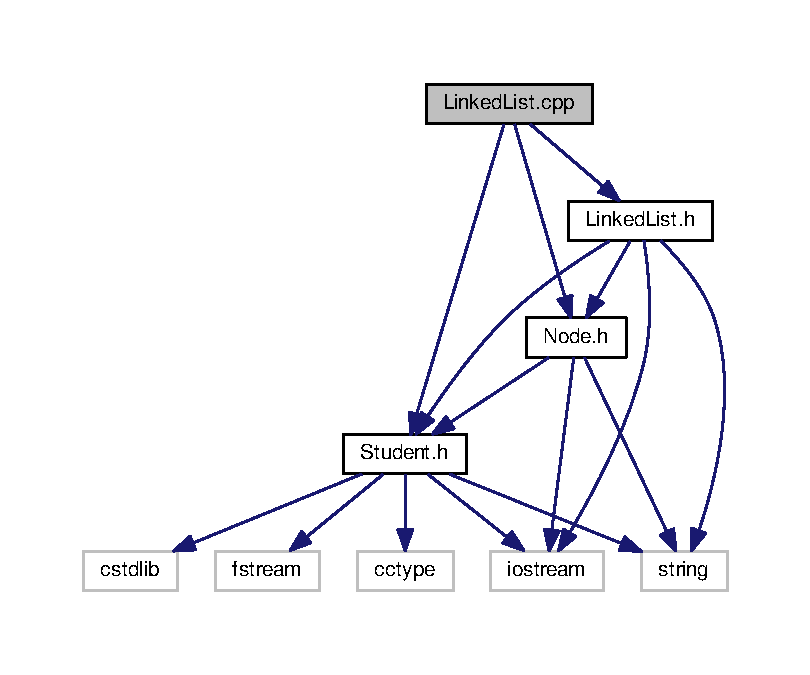
\includegraphics[width=350pt]{LinkedList_8cpp__incl}
\end{center}
\end{figure}

\hypertarget{LinkedList_8h}{}\section{Linked\+List.\+h File Reference}
\label{LinkedList_8h}\index{Linked\+List.\+h@{Linked\+List.\+h}}
{\ttfamily \#include $<$iostream$>$}\\*
{\ttfamily \#include $<$string$>$}\\*
{\ttfamily \#include \char`\"{}Student.\+h\char`\"{}}\\*
{\ttfamily \#include \char`\"{}Node.\+h\char`\"{}}\\*
Include dependency graph for Linked\+List.\+h\+:
\nopagebreak
\begin{figure}[H]
\begin{center}
\leavevmode
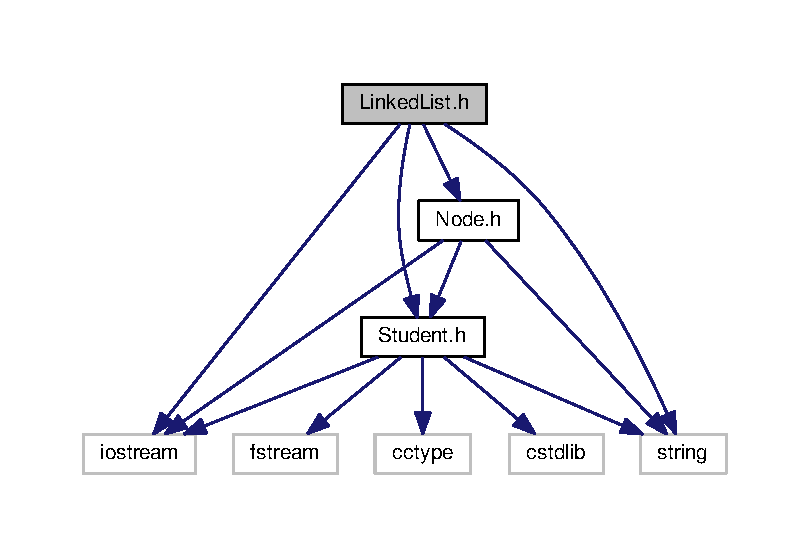
\includegraphics[width=350pt]{LinkedList_8h__incl}
\end{center}
\end{figure}
This graph shows which files directly or indirectly include this file\+:
\nopagebreak
\begin{figure}[H]
\begin{center}
\leavevmode
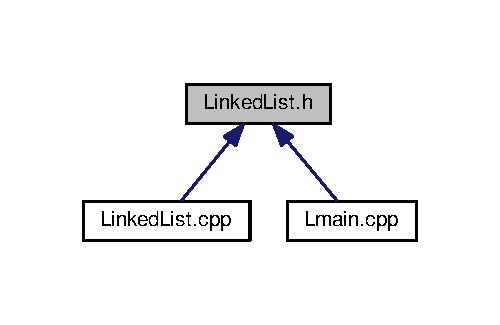
\includegraphics[width=240pt]{LinkedList_8h__dep__incl}
\end{center}
\end{figure}
\subsection*{Classes}
\begin{DoxyCompactItemize}
\item 
class \hyperlink{classLinkedList}{Linked\+List$<$ T $>$}
\end{DoxyCompactItemize}

\hypertarget{Lmain_8cpp}{}\section{Lmain.\+cpp File Reference}
\label{Lmain_8cpp}\index{Lmain.\+cpp@{Lmain.\+cpp}}
{\ttfamily \#include \char`\"{}Student.\+h\char`\"{}}\\*
{\ttfamily \#include \char`\"{}Node.\+h\char`\"{}}\\*
{\ttfamily \#include \char`\"{}Linked\+List.\+h\char`\"{}}\\*
{\ttfamily \#include $<$fstream$>$}\\*
Include dependency graph for Lmain.\+cpp\+:
\nopagebreak
\begin{figure}[H]
\begin{center}
\leavevmode
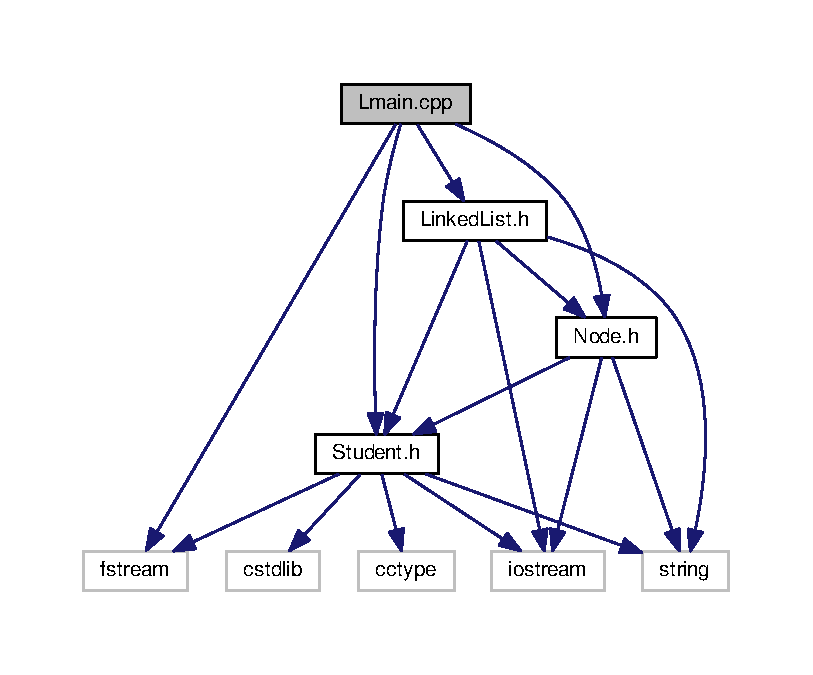
\includegraphics[width=350pt]{Lmain_8cpp__incl}
\end{center}
\end{figure}
\subsection*{Functions}
\begin{DoxyCompactItemize}
\item 
void \hyperlink{Lmain_8cpp_a70ec1382d8ba4ede7bc41284e71ba46f}{create\+Student} (string \&f, string \&l, char \&m, int \&ssn, int \&a)
\item 
void \hyperlink{Lmain_8cpp_a384998e9dc63c57a1ab89dba2cfb8d02}{set\+Up} (\hyperlink{classLinkedList}{Linked\+List}$<$ \hyperlink{classStudent}{Student} $>$ \&list)
\item 
void \hyperlink{Lmain_8cpp_a35b314eba9ac1561de239605dd8289f9}{finish} (\hyperlink{classLinkedList}{Linked\+List}$<$ \hyperlink{classStudent}{Student} $>$ \&list)
\item 
int \hyperlink{Lmain_8cpp_ae66f6b31b5ad750f1fe042a706a4e3d4}{main} ()
\end{DoxyCompactItemize}


\subsection{Function Documentation}
\index{Lmain.\+cpp@{Lmain.\+cpp}!create\+Student@{create\+Student}}
\index{create\+Student@{create\+Student}!Lmain.\+cpp@{Lmain.\+cpp}}
\subsubsection[{\texorpdfstring{create\+Student(string \&f, string \&l, char \&m, int \&ssn, int \&a)}{createStudent(string &f, string &l, char &m, int &ssn, int &a)}}]{\setlength{\rightskip}{0pt plus 5cm}void create\+Student (
\begin{DoxyParamCaption}
\item[{string \&}]{f, }
\item[{string \&}]{l, }
\item[{char \&}]{m, }
\item[{int \&}]{ssn, }
\item[{int \&}]{a}
\end{DoxyParamCaption}
)}\hypertarget{Lmain_8cpp_a70ec1382d8ba4ede7bc41284e71ba46f}{}\label{Lmain_8cpp_a70ec1382d8ba4ede7bc41284e71ba46f}

\begin{DoxyCode}
83 \{
84    cout << endl <<\textcolor{stringliteral}{"Enter first name: "};
85    cin >> f;
86    cout << \textcolor{stringliteral}{"Enter last name: "};
87    cin >> l;
88    cout << \textcolor{stringliteral}{"Enter middle initial: "};
89    cin >> m;
90    cout << \textcolor{stringliteral}{"Enter social security number: "};
91    cin >> ssn;
92    cout << \textcolor{stringliteral}{"Enter age: "};
93    cin >> a;
94 \}
\end{DoxyCode}
\index{Lmain.\+cpp@{Lmain.\+cpp}!finish@{finish}}
\index{finish@{finish}!Lmain.\+cpp@{Lmain.\+cpp}}
\subsubsection[{\texorpdfstring{finish(\+Linked\+List$<$ Student $>$ \&list)}{finish(LinkedList< Student > &list)}}]{\setlength{\rightskip}{0pt plus 5cm}void finish (
\begin{DoxyParamCaption}
\item[{{\bf Linked\+List}$<$ {\bf Student} $>$ \&}]{list}
\end{DoxyParamCaption}
)}\hypertarget{Lmain_8cpp_a35b314eba9ac1561de239605dd8289f9}{}\label{Lmain_8cpp_a35b314eba9ac1561de239605dd8289f9}

\begin{DoxyCode}
121 \{
122    ofstream out\_stream;
123 
124    out\_stream.open(\textcolor{stringliteral}{"StudentData.txt"}); \textcolor{comment}{// opens file StudentData.txt                                       
                                                                                                       }
125    \textcolor{keywordflow}{if}(out\_stream.fail()) \textcolor{comment}{// If the file cannot open, the program ends                                      
                                                                                                       }
126    \{
127       cout << \textcolor{stringliteral}{"Output file opening failed.\(\backslash\)n"};
128       exit(1);
129    \}
130 
131    \hyperlink{classNode}{Node<Student>}* curr = list.\hyperlink{classLinkedList_af59e26b062e8e9549974adfa5bb51eb2}{getHead}();
132    \textcolor{keywordflow}{while}(curr) \textcolor{comment}{//goes through all Nodes                                                                    
                                                                                                       }
133    \{
134       curr -> getStudent().print(out\_stream); \textcolor{comment}{//prints Student information into the file                   
                                                                                                       }
135       curr = curr -> \hyperlink{classNode_af8f2d178f274dd254e6e1965971f0fd0}{getNext}(); \textcolor{comment}{//goes to the next Node in the list                                 
                                                                                                              }
136    \}
137 
138    out\_stream.close(); \textcolor{comment}{// closes the file                                                                  
                                                                                                       }
139 \}
\end{DoxyCode}


Here is the call graph for this function\+:
\nopagebreak
\begin{figure}[H]
\begin{center}
\leavevmode
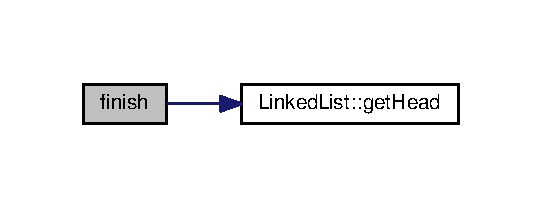
\includegraphics[width=260pt]{Lmain_8cpp_a35b314eba9ac1561de239605dd8289f9_cgraph}
\end{center}
\end{figure}


\index{Lmain.\+cpp@{Lmain.\+cpp}!main@{main}}
\index{main@{main}!Lmain.\+cpp@{Lmain.\+cpp}}
\subsubsection[{\texorpdfstring{main()}{main()}}]{\setlength{\rightskip}{0pt plus 5cm}int main (
\begin{DoxyParamCaption}
{}
\end{DoxyParamCaption}
)}\hypertarget{Lmain_8cpp_ae66f6b31b5ad750f1fe042a706a4e3d4}{}\label{Lmain_8cpp_ae66f6b31b5ad750f1fe042a706a4e3d4}

\begin{DoxyCode}
24 \{
25    \hyperlink{classLinkedList}{LinkedList<Student>} list;
26    \hyperlink{classNode}{Node<Student>}* nPtr;
27    \textcolor{keywordtype}{string} f, l;
28    \textcolor{keywordtype}{int} n, ssn, a, count = -1;
29    \textcolor{keywordtype}{char} ans = \textcolor{charliteral}{'y'}, m;
30    \textcolor{keywordtype}{bool} del;
31 
32    \textcolor{comment}{//setUp(list); //updates list with info from the file                                                   
                                                                                                       }
33    cout << endl << \textcolor{stringliteral}{"Do you want to add students to your list? y/n: "};
34    cin >> ans;
35    \textcolor{keywordflow}{while}(ans == \textcolor{charliteral}{'y'} || ans == \textcolor{charliteral}{'Y'})
36    \{
37       \hyperlink{Lmain_8cpp_a70ec1382d8ba4ede7bc41284e71ba46f}{createStudent}(f, l, m, ssn, a);
38       nPtr = \textcolor{keyword}{new} \hyperlink{classNode_a0ac1d44cfe588be564acf25485029bd8}{Node}(f, l, m, ssn, a); \textcolor{comment}{//creates new Node (which nPtr points to) with the Student
       object just created                                                                                      }
39       list.\hyperlink{classLinkedList_ac2f92598858e9ba02af8722fba803c53}{append}(nPtr); \textcolor{comment}{//appends the newly created Node to the list                                
                                                                                                             }
40       cout << \textcolor{stringliteral}{"\(\backslash\)nAdd a new student to the list? y/n: "};
41       cin >> ans;
42    \} \textcolor{comment}{//Nodes will be created until user does not enter y or Y                                              
                                                                                                       }
43 
44    cout << \textcolor{stringliteral}{"Student list ("} << list.\hyperlink{classLinkedList_ae04dbbcae32f8fb03dce3e174854981f}{getNumNode}() << \textcolor{stringliteral}{" students):"} << endl << endl;
45    list.\hyperlink{classLinkedList_afddb5dbcc39e687add40de41b975cd8d}{display}(); \textcolor{comment}{//displays list                                                                  
                                                                                                              }
46 
47    \textcolor{keywordflow}{do}
48    \{
49       count++; \textcolor{comment}{//counts to see how many times deleteNode() was called                                      
                                                                                                       }
50       del = list.deleteNode(\textcolor{stringliteral}{"Christine"}); \textcolor{comment}{//deletes all Nodes with the name Christine                      
                                                                                                       }
51    \}\textcolor{keywordflow}{while}(del); \textcolor{comment}{//continue to delete Nodes until there are no more Christines in the list                  
                                                                                                       }
52    \textcolor{keywordflow}{if}(count > 0) \textcolor{comment}{//if any Nodes were deleted, the list will print again                                    
                                                                                                       }
53    \{
54       cout << \textcolor{stringliteral}{"\(\backslash\)nAfter Christine has been deleted from list:"} << endl << endl;
55       list.\hyperlink{classLinkedList_afddb5dbcc39e687add40de41b975cd8d}{display}();
56    \}
57 \textcolor{comment}{/*                                                                                                         
                                                                                                       }
58 \textcolor{comment}{   LinkedList bubble(list); //create copy of list                                                          
                                                                                                       }
59 \textcolor{comment}{   cout << "\(\backslash\)ndisplaying copied list:\(\backslash\)n\(\backslash\)n";}
60 \textcolor{comment}{   bubble.display();                                                                                       
                                                                                                       }
61 \textcolor{comment}{   bubble.bubbleSort(); //sorts the new list by bubble sort                                                
                                                                                                       }
62 \textcolor{comment}{   cout << "\(\backslash\)ndisplaying bubble sorted list:\(\backslash\)n\(\backslash\)n";                                                         
                                                                                                       }
63 \textcolor{comment}{   bubble.display();                                                                                       
                                                                                                       }
64 \textcolor{comment}{                                                                                                           
                                                                                                       }
65 \textcolor{comment}{   LinkedList selection(list); //create copy of list                                                       
                                                                                                       }
66 \textcolor{comment}{   cout << "\(\backslash\)ndisplaying copied list:\(\backslash\)n\(\backslash\)n";                                                                
                                                                                                       }
67 \textcolor{comment}{   selection.display();                                                                                    
                                                                                                       }
68 \textcolor{comment}{   selection.selectionSort(); //sorts new list by selection sort                                           
                                                                                                       }
69 \textcolor{comment}{   cout << "\(\backslash\)ndisplaying selection sorted list:\(\backslash\)n\(\backslash\)n";                                                      
                                                                                                       }
70 \textcolor{comment}{   selection.display();                                                                                    
                                                                                                       }
71 \textcolor{comment}{*/}
72    \hyperlink{classLinkedList}{LinkedList} L2(list, \textcolor{keyword}{true}); \textcolor{comment}{//creates a copy of list, but sorted                               
                                                                                                                 }
73    cout << \textcolor{stringliteral}{"\(\backslash\)nSORTED list copied from original list ("}  << L2.getNumNode() << \textcolor{stringliteral}{" students):"} << endl << endl
      ;
74    L2.display();
75 
76    \textcolor{comment}{//finish(list); //save Students from L2 into the file                                                   
                                                                                                       }
77    \textcolor{keywordflow}{return} 0;
78 \}
\end{DoxyCode}


Here is the call graph for this function\+:
\nopagebreak
\begin{figure}[H]
\begin{center}
\leavevmode
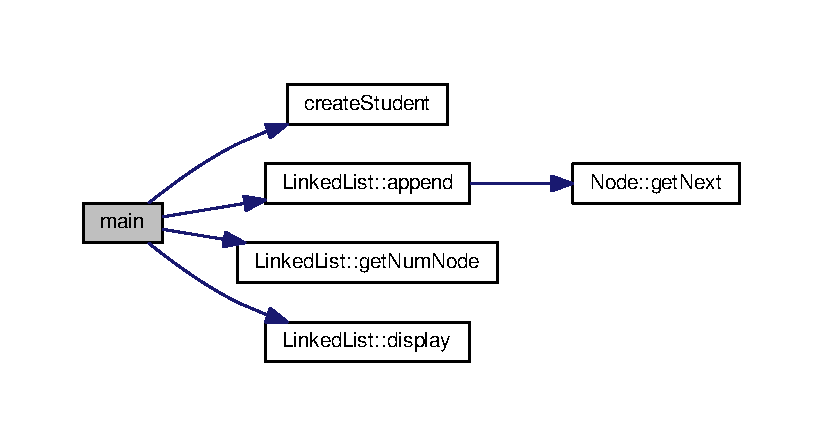
\includegraphics[width=350pt]{Lmain_8cpp_ae66f6b31b5ad750f1fe042a706a4e3d4_cgraph}
\end{center}
\end{figure}


\index{Lmain.\+cpp@{Lmain.\+cpp}!set\+Up@{set\+Up}}
\index{set\+Up@{set\+Up}!Lmain.\+cpp@{Lmain.\+cpp}}
\subsubsection[{\texorpdfstring{set\+Up(\+Linked\+List$<$ Student $>$ \&list)}{setUp(LinkedList< Student > &list)}}]{\setlength{\rightskip}{0pt plus 5cm}void set\+Up (
\begin{DoxyParamCaption}
\item[{{\bf Linked\+List}$<$ {\bf Student} $>$ \&}]{list}
\end{DoxyParamCaption}
)}\hypertarget{Lmain_8cpp_a384998e9dc63c57a1ab89dba2cfb8d02}{}\label{Lmain_8cpp_a384998e9dc63c57a1ab89dba2cfb8d02}

\begin{DoxyCode}
97 \{
98    \hyperlink{classStudent}{Student}* sPtr;
99    \hyperlink{classStudent}{Student} s;
100    \hyperlink{classNode}{Node<Student>}* nPtr;
101    ifstream in\_stream;
102    \textcolor{keywordtype}{string} temp;
103 
104    in\_stream.open(\textcolor{stringliteral}{"StudentData.txt"}); \textcolor{comment}{// opens file StudentData.txt                                        
                                                                                                       }
105    \textcolor{keywordflow}{if}(in\_stream.fail()) \textcolor{comment}{// If the file does not open, the program will exit                                
                                                                                                       }
106    \{
107       cout << \textcolor{stringliteral}{"Input file opening failed.\(\backslash\)n"};
108       exit(1);
109    \}
110 
111    \textcolor{keywordflow}{while}(in\_stream >> s) \textcolor{comment}{// reads in the values from the file to the end of the file                       
                                                                                                       }
112    \{
113       sPtr = \textcolor{keyword}{new} \hyperlink{classStudent}{Student}(s);
114       nPtr = \textcolor{keyword}{new} \hyperlink{classNode_a0ac1d44cfe588be564acf25485029bd8}{Node}(sPtr);
115       list.\hyperlink{classLinkedList_ac2f92598858e9ba02af8722fba803c53}{append}(nPtr);
116    \}
117    in\_stream.close(); \textcolor{comment}{// closes the file                                                                   
                                                                                                       }
118 \}
\end{DoxyCode}


Here is the call graph for this function\+:
\nopagebreak
\begin{figure}[H]
\begin{center}
\leavevmode
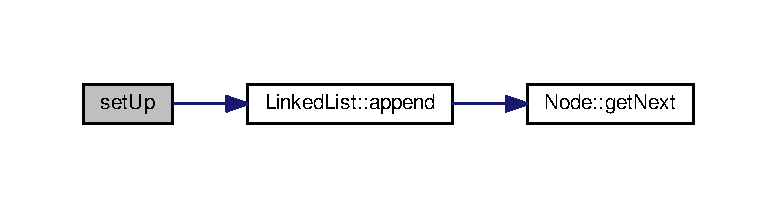
\includegraphics[width=350pt]{Lmain_8cpp_a384998e9dc63c57a1ab89dba2cfb8d02_cgraph}
\end{center}
\end{figure}



\hypertarget{Node_8cpp}{}\section{Node.\+cpp File Reference}
\label{Node_8cpp}\index{Node.\+cpp@{Node.\+cpp}}
{\ttfamily \#include \char`\"{}Node.\+h\char`\"{}}\\*
{\ttfamily \#include \char`\"{}Student.\+h\char`\"{}}\\*
Include dependency graph for Node.\+cpp\+:
\nopagebreak
\begin{figure}[H]
\begin{center}
\leavevmode
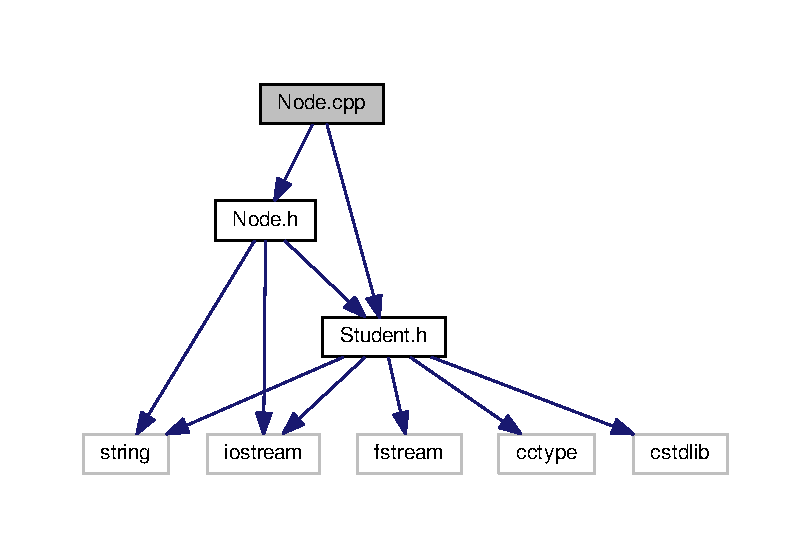
\includegraphics[width=350pt]{Node_8cpp__incl}
\end{center}
\end{figure}

\hypertarget{Node_8h}{}\section{Node.\+h File Reference}
\label{Node_8h}\index{Node.\+h@{Node.\+h}}
{\ttfamily \#include $<$iostream$>$}\\*
{\ttfamily \#include $<$string$>$}\\*
{\ttfamily \#include \char`\"{}Student.\+h\char`\"{}}\\*
Include dependency graph for Node.\+h\+:
\nopagebreak
\begin{figure}[H]
\begin{center}
\leavevmode
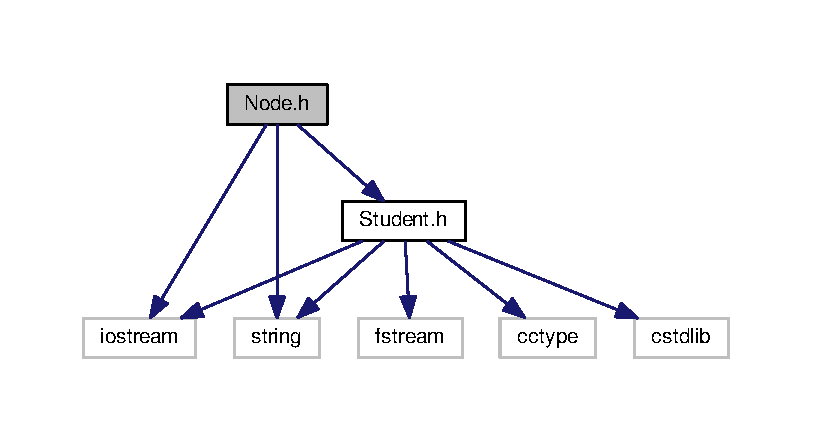
\includegraphics[width=350pt]{Node_8h__incl}
\end{center}
\end{figure}
This graph shows which files directly or indirectly include this file\+:
\nopagebreak
\begin{figure}[H]
\begin{center}
\leavevmode
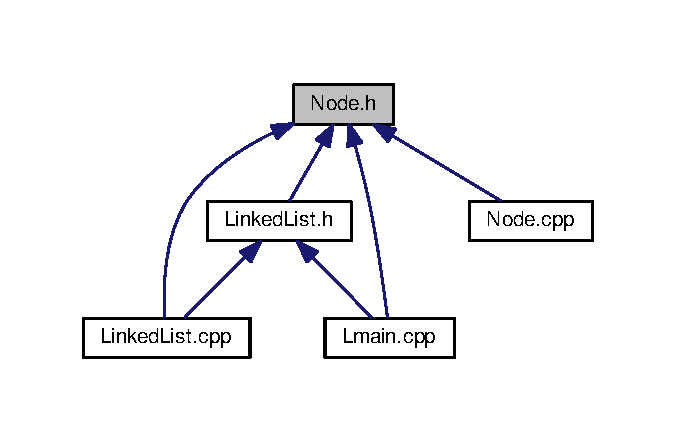
\includegraphics[width=350pt]{Node_8h__dep__incl}
\end{center}
\end{figure}
\subsection*{Classes}
\begin{DoxyCompactItemize}
\item 
class \hyperlink{classNode}{Node$<$ T $>$}
\end{DoxyCompactItemize}

\hypertarget{Student_8cpp}{}\section{Student.\+cpp File Reference}
\label{Student_8cpp}\index{Student.\+cpp@{Student.\+cpp}}
{\ttfamily \#include \char`\"{}Student.\+h\char`\"{}}\\*
Include dependency graph for Student.\+cpp\+:
\nopagebreak
\begin{figure}[H]
\begin{center}
\leavevmode
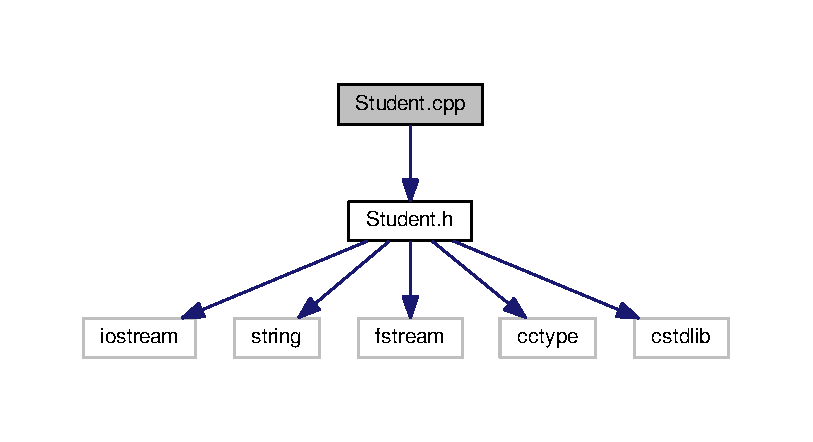
\includegraphics[width=350pt]{Student_8cpp__incl}
\end{center}
\end{figure}
\subsection*{Functions}
\begin{DoxyCompactItemize}
\item 
ostream \& \hyperlink{Student_8cpp_a8ed16acc8384ea29641694cb182ac764}{operator$<$$<$} (ostream \&outs, const \hyperlink{classStudent}{Student} \&s)
\item 
istream \& \hyperlink{Student_8cpp_a2d76cee765e6e0d66e66a27d10fa0a68}{operator$>$$>$} (istream \&ins, \hyperlink{classStudent}{Student} \&s)
\end{DoxyCompactItemize}


\subsection{Function Documentation}
\index{Student.\+cpp@{Student.\+cpp}!operator$<$$<$@{operator$<$$<$}}
\index{operator$<$$<$@{operator$<$$<$}!Student.\+cpp@{Student.\+cpp}}
\subsubsection[{\texorpdfstring{operator$<$$<$(ostream \&outs, const Student \&s)}{operator<<(ostream &outs, const Student &s)}}]{\setlength{\rightskip}{0pt plus 5cm}ostream\& operator$<$$<$ (
\begin{DoxyParamCaption}
\item[{ostream \&}]{outs, }
\item[{const {\bf Student} \&}]{s}
\end{DoxyParamCaption}
)}\hypertarget{Student_8cpp_a8ed16acc8384ea29641694cb182ac764}{}\label{Student_8cpp_a8ed16acc8384ea29641694cb182ac764}

\begin{DoxyCode}
65 \{
66    cout << \textcolor{stringliteral}{"Student:\(\backslash\)t\(\backslash\)t  "} << s.\hyperlink{classStudent_a6c934004d6a468a354916bcf0f998190}{lname} << \textcolor{stringliteral}{", "} << s.\hyperlink{classStudent_a333c7d227c87fdfa821d0232e21f9006}{fname} << \textcolor{stringliteral}{" "} << s.
      \hyperlink{classStudent_afd8d4557f2ac6bb7681c32e691248328}{mi} << endl;
67    cout << \textcolor{stringliteral}{"Social Security number:\(\backslash\)t  "} << s.\hyperlink{classStudent_aa7181a8aac86888176481f901bee2cbd}{ssn} << endl;
68    cout << \textcolor{stringliteral}{"Age:\(\backslash\)t\(\backslash\)t\(\backslash\)t  "} << s.\hyperlink{classStudent_a552a431a43ffc545d180424597d51f97}{age} << endl;
69    cout << \textcolor{stringliteral}{"------------------------------------------------------"} << endl;
70 
71    \textcolor{keywordflow}{return} outs;
72 \}
\end{DoxyCode}
\index{Student.\+cpp@{Student.\+cpp}!operator$>$$>$@{operator$>$$>$}}
\index{operator$>$$>$@{operator$>$$>$}!Student.\+cpp@{Student.\+cpp}}
\subsubsection[{\texorpdfstring{operator$>$$>$(istream \&ins, Student \&s)}{operator>>(istream &ins, Student &s)}}]{\setlength{\rightskip}{0pt plus 5cm}istream\& operator$>$$>$ (
\begin{DoxyParamCaption}
\item[{istream \&}]{ins, }
\item[{{\bf Student} \&}]{s}
\end{DoxyParamCaption}
)}\hypertarget{Student_8cpp_a2d76cee765e6e0d66e66a27d10fa0a68}{}\label{Student_8cpp_a2d76cee765e6e0d66e66a27d10fa0a68}

\begin{DoxyCode}
75 \{
76    ins >> s.\hyperlink{classStudent_a333c7d227c87fdfa821d0232e21f9006}{fname} >> s.\hyperlink{classStudent_a6c934004d6a468a354916bcf0f998190}{lname} >> s.\hyperlink{classStudent_afd8d4557f2ac6bb7681c32e691248328}{mi} >> s.\hyperlink{classStudent_aa7181a8aac86888176481f901bee2cbd}{ssn} >> s.\hyperlink{classStudent_a552a431a43ffc545d180424597d51f97}{age};
77 \}
\end{DoxyCode}

\hypertarget{Student_8h}{}\section{Student.\+h File Reference}
\label{Student_8h}\index{Student.\+h@{Student.\+h}}
{\ttfamily \#include $<$iostream$>$}\\*
{\ttfamily \#include $<$string$>$}\\*
{\ttfamily \#include $<$fstream$>$}\\*
{\ttfamily \#include $<$cctype$>$}\\*
{\ttfamily \#include $<$cstdlib$>$}\\*
Include dependency graph for Student.\+h\+:
\nopagebreak
\begin{figure}[H]
\begin{center}
\leavevmode
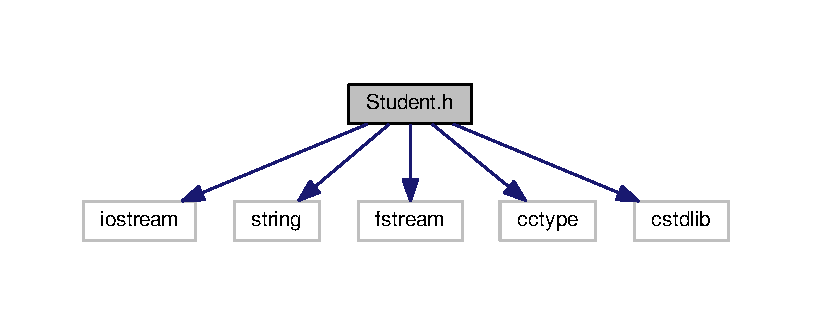
\includegraphics[width=350pt]{Student_8h__incl}
\end{center}
\end{figure}
This graph shows which files directly or indirectly include this file\+:
\nopagebreak
\begin{figure}[H]
\begin{center}
\leavevmode
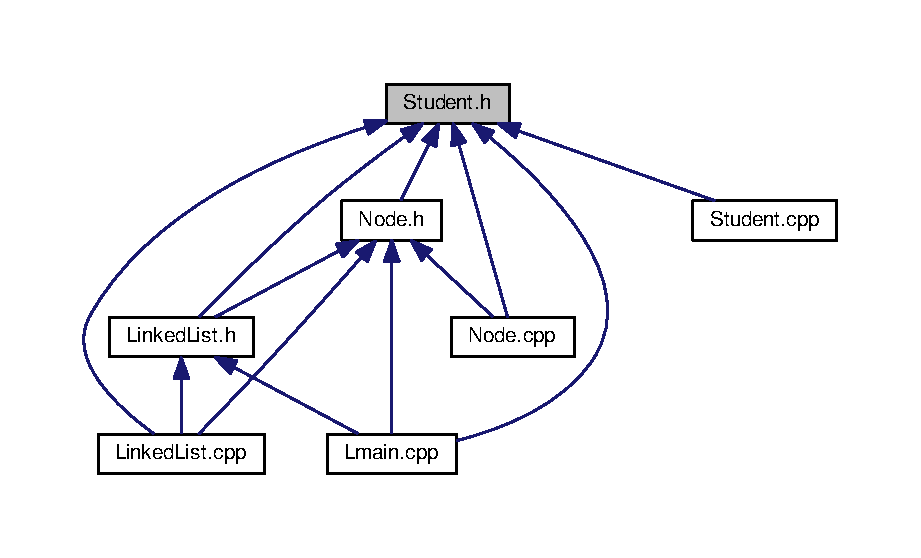
\includegraphics[width=308pt]{Student_8h__dep__incl}
\end{center}
\end{figure}
\subsection*{Classes}
\begin{DoxyCompactItemize}
\item 
class \hyperlink{classStudent}{Student}
\end{DoxyCompactItemize}

%--- End generated contents ---

% Index
\backmatter
\newpage
\phantomsection
\clearemptydoublepage
\addcontentsline{toc}{chapter}{Index}
\printindex

\end{document}
